%%%%%%%%%%%%%%%%%%%%%%%%%%%%%%%%%%%%%%%%%%%%%%%%%%%%%%%%%%%%%%%
%
% Welcome to Overleaf --- just edit your LaTeX on the left,
% and we'll compile it for you on the right. If you open the
% 'Share' menu, you can invite other users to edit at the same
% time. See www.overleaf.com/learn for more info. Enjoy!
%
%%%%%%%%%%%%%%%%%%%%%%%%%%%%%%%%%%%%%%%%%%%%%%%%%%%%%%%%%%%%%%%
\documentclass{article}
\usepackage{tcolorbox}
\usepackage{soul, color, xcolor}

\usepackage{geometry}
    \geometry{a4paper,scale=0.779}
   \title{\textbf{Supplementary Material \& Example Prompts: \\
   Large Language Models as Efficient Reward Function Searchers for Custom-Environment Multi-objective Reinforcement learning}}    
   % \title{\textbf{Supplementary Material \& Example Prompts: \\
   % ERFSL: An Efficient Reward Function Searcher via Large Language Models for Custom-Environment Multi-Objective Reinforcement Learning}}
   \author{}
   \date{}
\usepackage[T1]{fontenc}
\usepackage{minted}
\usepackage{amsmath}
\begin{document}
   \maketitle
   In this supplementary material, we first briefly present the system models and experimental settings. Then, we present examples of prompts of ERFSL LLM-aided reward function search framework, along with the answers generated by LLMs. All LLM-generated outputs are based on the \verb|gpt-4o-2024-08-06| version of OpenAI's LLM, with parameters \verb|temperature=0.5| and \verb|Top P=1|. % We will update the automatic weight adjusting code in October 2024.
   
  Notice that, unlike the prompts used in code implementation, most prompts in this appendix omit the demands for structured output, such as those for reward code matching, and so on.
   
\tableofcontents
\newpage
\section{System Models and Experimental Settings} 

The environment used for our experiment is a simplified version of our previous work \cite{1}, omitting vortexes and certain underwater disturbances. We briefly introduce the system model of the multi-AUV data collection task, then present the experimental settings.

\subsection{System Model of The Multi-AUV Data Collection Task}
\subsubsection{Underwater Data Collection Model}
The system model of the multi-AUV data collection task utilized in this study is illustrated in Fig. 1. Consider an environment containing $N$ task-performing AUVs and $\lambda$ IoUT sensor nodes, where the AUVs are denoted by set $AUVs=\{AUV_1,AUV_2,\ldots,AUV_N\}$. These AUVs receive status information of IoUT device nodes from the base station on the sea surface, which enables them to identify the nodes requiring data collection. The IoUT nodes are represented by set $\Phi=\{\Phi_{1},\Phi_{2},\ldots,\Phi_{\lambda}\}$, comprising $\mu$ ordinary nodes $\Phi_{k}^{\mathrm{N}}=\{\Phi_{k_{1}}^{\mathrm{N}},\Phi_{k_{2}}^{\mathrm{N}},\ldots,\Phi_{k_{\mu}}^{\mathrm{N}}\}$ and $\nu$ data-collecting nodes $\Phi_{j}^{\mathcal{F}}=\{\Phi_{o_{1}}^{\mathcal{F}},\Phi_{o_{2}}^{\mathcal{F}},\ldots,\Phi_{o_{\nu}}^{\mathcal{F}}\}$. The components of the system are described as follows.

\textbf{Ordinary Nodes:} The underwater nodes equipped with fundamental functions including signal reception, data storage, and signal transmission. These nodes do not have data backlog and do not require data collection capabilities.

\textbf{Data-Collecting Nodes:} Underwater nodes that require data collection due to a certain degree of data backlog.

\textbf{AUVs:} AUVs equipped with communication devices, sensors, mechanical arms, and charging/storage equipment. In this work, the role of the AUV is to locate nodes within the IoUT network and perform data collection tasks.

\textbf{Surface Base Stations:} Information transmission and storage centers located on the sea surface or on land, responsible for the overall coordination of multi-AUV underwater data collection task.


During data collection operations, AUVs work collaboratively to locate nodes that require data collection. Considering that ocean turbulence significantly impacts the movement and energy consumption of AUVs, they must avoid turbulent areas during operation to optimize their trajectories.

\begin{figure}[!htb]
    \centering
    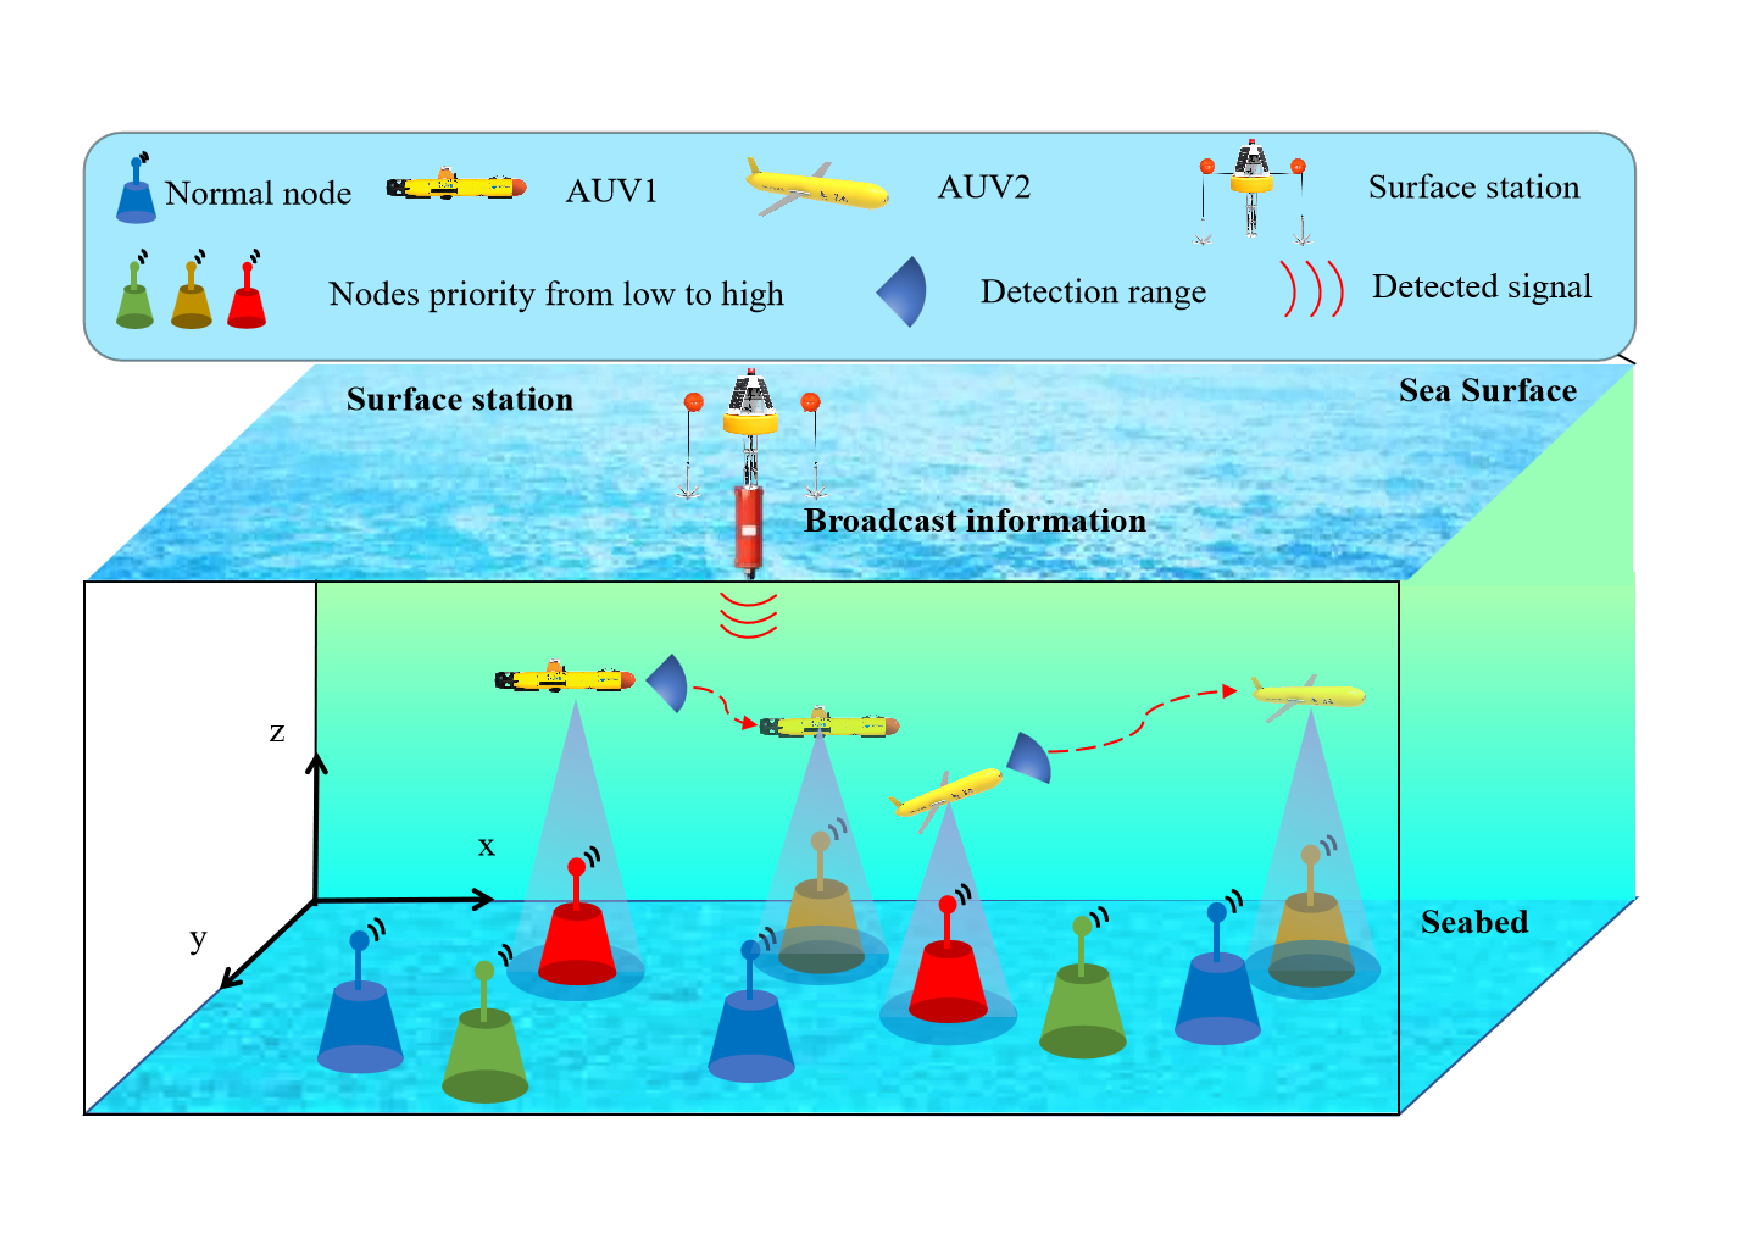
\includegraphics[width=0.788\linewidth]{system_model.pdf}
    \caption{The system model of the multi-AUV data collection task.}
    \label{1}
\end{figure}


\subsubsection{AUV Communication Model}\label{se:3.3}

During the multi-AUV data collection task, AUVs detect sensor nodes using their onboard sonar systems. Concurrently, communication between AUVs is also facilitated through sonar equipment. These processes can be uniformly modeled using the underwater environment sonar equation
\begin{equation}\label{eq:6}
EM=SL+TS+DI-NL-DT-2TL(d,f),
\end{equation}
where $SL$, $TS$, $DI$, $NL$, and $TL(d,f)$ represent the source level, target strength, directivity index, ambient noise level, and transmission loss, respectively. $DT$ and $EM$ denote the active sonar detection threshold and the echo excess, respectively. $TL(d,f)$ is related to the detection radius $d$ and the center frequency $f$, satisfying the following equation:
\begin{equation}\label{eq:7}
TL(d,f)=20\mathrm{log}(d)+\frac{d\kappa(f)}{1000},
\end{equation}
where $\kappa(f)$ represents the absorption coefficient, calculated according to the Thorp formula
\begin{equation}\label{eq:8}
\kappa(f)= 0.11\frac{f^{2}}{1+ f^{2}}+ 44 \frac{f^{2}}{4100+ f^{2}}+ 2.75\times10^{-4} f^{2}+0.003.
\end{equation}

In the underwater environment, the total noise $N_l$ consists of turbulence noise $N_t$, shipping noise $N_s$, wind noise $N_w$, and thermal noise $N_{th}$. These noises can be represented by Gaussian statistics, and the total power spectral density (PSD) of $N_l$ is
\begin{equation}\label{eq:9}
N_l(f)=N_t(f)+N_s(f)+N_w(f)+N_{th}(f).
\end{equation}

The noise component in Equation 8 can be expressed as
\begin{equation}\label{eq:10}
\begin{cases}
10\mathrm{log}N_t(f)=17-30\mathrm{log}f,\\10\mathrm{log}N_s(f)=30+20s+\log\left(\frac{f^{26}}{(f+0.03)^{60}}\right),\\10\mathrm{log}N_w(f)=50+7.5\omega^{\frac{1}{2}}+20\mathrm{log}\left(\frac{f}{(f+0.4)^{2}}\right),\\10\mathrm{log}N_{th}(f)=- 15+20\mathrm{log}f,
\end{cases}
\end{equation}
where $s\in(0,1)$ represents the activity factor, and $\omega$ is the wind speed with the unit of m/s.

\subsubsection{AUV Energy Consumption Model}\label{se:3.4}
The energy consumption of the AUV arises from two primary sources: the hovering energy consumption $\mathcal{M}_j^h$, and the traveling energy consumption $\mathcal{M}_j^m$. According to classical fluid dynamics, the drag experienced by the AUV while hovering underwater can be expressed as
\begin{equation}\label{eq:11}
\tau_j^h=\frac{\rho_s\|v_c(\mathcal{r}_j^t)\|_2^2C_a\mathcal{U}_d}{2}.
\end{equation}

The resistance during navigation can be expressed as
\begin{equation}\label{eq:12}
\tau_j^m=\frac{\rho_s\|v_k(\mathcal{r}_j^t)\|_2^2C_a\mathcal{U}_d}{2},
\end{equation}
where $\rho_s$ represents the density of seawater, while $C_a$ and $\mathcal{U}_d$ denote the drag coefficient and frontal area of the AUV, respectively. And $\mathcal{r}_j^t$ is the position vector of the AUV $j$ at time $t$. Additionally, $v_c(\mathcal{r}_j^t)$ and $v_k(\mathcal{r}_j^t)$ represent the flow velocity and relative velocity at position $\mathcal{r}_j^t$, respectively. Therefore, the power consumption of the AUV $j$ hovering at the $\hbar$-th node can be calculated as follows:
\begin{equation}\label{eq:13}
P_j^h[\hbar]=\frac{\tau_j^h[\hbar]\|v_c(\mathcal{r}_j^\hbar)\|_2^2}{\vartheta},
\end{equation}
where $\vartheta$ is the electrical conversion efficiency.

Considering the practical situation, the relative velocity at different positions varies as the AUV moves from the $\hbar$-th node to the $(\hbar+1)$-th node. Hence, it is inappropriate to use the velocity at a single fixed point to calculate the energy consumption of the AUV during its movement. To address this issue, we use the average relative velocity at the starting point, midpoint, and endpoint of the trajectory to calculate the energy consumption. Taking the process of the AUV moving from the $\hbar$-th node to the $(\hbar+1)$-th node as an example, the average relative velocity is expressed as follows:
\begin{equation}\label{eq:14}
\overline{\boldsymbol{v}_k}\big(\mathcal{r}_j^\hbar\big)=\frac{\boldsymbol{v}_k\big(\mathcal{r}_j^\hbar\big)+\boldsymbol{v}_k\big(\mathcal{r}_j^{\hbar m}\big)+\boldsymbol{v}_k\big(\mathcal{r}_j^{\hbar+1}\big)}{3},
\end{equation}
where $\mathcal{r}_j^{\hbar m}$ denotes the position vector of the intermediate point of the trajectory. Therefore, the power consumption of the AUV in this motion trajectory is
\begin{equation}\label{eq:15}
P_j^m[\hbar]=\frac{\rho_s\|\overline{v_k}(\mathcal{r}_j^\hbar)\|_2^2C_a\mathcal{U}_d\|\overline{v_k}(\mathcal{r}_j^\hbar)\|_2^2}{2\zeta}.
\end{equation}

Based on the above analysis, the total energy consumption of AUV $j$ can be concluded as follows
\begin{equation}\label{eq:16}
E_{j}=\sum_{i=1}^{M}\sum_{\hbar=1}^{\Phi_{o}^{F_{j}}}\chi_{j,i} [\hbar]P_{j}^{h}[\hbar]\pi_{j,i}[\hbar]+\sum_{\hbar=1}^{\Phi_{o}^{F_{j}}}P_{j}^{m}[\hbar]t_{j}^{m}[\hbar],
\end{equation}
where $M$ represents the set of all nodes, while $\chi_{j,i}[\hbar]=1$ denotes the event that the AUV $j$ hovers over node $i$ for the $\hbar$-th time, and conversely, $\chi_{j,i}[\hbar]=0$. $\pi_{j,i}[\hbar]$ represents the hovering time over the node, $\Phi_{o}^{F_{j}}$ denotes the set of hovering points of AUV $j$, and $t_{j}^{m}[\hbar]$ represents the time required to move from the $\hbar$-th node to the $\hbar+1$-th node.

\subsubsection{Node Selection Model}
Before the AUV initiates data collection from IoUT nodes, it is essential to determine the priority based on the urgency of data collection required by each node. The priority $\mathcal{Q}_{\hbar}^{j}(t)$ of data collection from a node is defined as follows:
\begin{equation}\mathcal{Q}_{\hbar}^{j}(t)=\frac{\mathcal{C}_{\hbar}(t)}{\mathcal{C}_{max}(\mathcal{N}_{\hbar}(t)+\varepsilon)}-\xi d_{\hbar}^{j}(t),\end{equation}
where $\mathcal{N}_{\hbar}(t)\in[0,\mathcal{N}_{\hbar}^{max}]$ is the channel capacity of node $\hbar$ at time $t$, $\mathcal{C}_\hbar(t)\in[0,\mathcal{C}_{max}]$ represents the data storage amount, and $\mathcal{C}_{max}$ denotes the maximum data storage capacity of the node. $d_{\hbar}^{j}(t)$ represents the relative distance between AUV $j$ and node $\hbar$ at time $t$, $\varepsilon$ denotes a constant to prevent calculation errors when $\mathcal{N}_{\hbar}(t)$ equals zero, and $\xi$ is a penalty factor. By calculating $\mathcal{Q}_{\hbar}^{j}(t)$, the AUV can prioritize collecting data from nodes with higher urgency while considering the relative distance, thereby improving the system's operational efficiency.


\subsection{Experimental Settings}
In the "Objectives of the Task" section of the prompt in Section 2 of this supplementary material, we present the main user requirements. The system model, state space, and action space adopted are consistent with those in \cite{1}. Compared to the paper \cite{1}, we limit the minimum value of the AUV speed so that the energy consumption cannot be lower than 50W. Additionally, the main experimental conditions and selected parameters are detailed as follows:
\begin{table*}[!ht]
    \centering
    \caption{Environmental Parameters.}
    \label{tab:3}
    %\begin{tabular}{m{4.5cm}|m{3.2cm}}
    \begin{tabular}{l|l}
    \hline
    \multicolumn{1}{c|}{Parameters} & \multicolumn{1}{c}{Values}\\
    \hline
    Numbers of AUVs & 2(\verb|state_dim=8,action_dim=2|) \\
    Experimental area & 120m$\times$ 120m \\
    Episode length & 1000s (1000 timesteps) \\
    The number of SNs (IoUT devices) & 40 \\
    Communication radius $R_r$ & 6m \\
    Target SN choosing parameter $\alpha$ & 0.0 \\
    \hline
    \end{tabular}
    \end{table*}

    \begin{table*}[!ht]
    \centering
    \caption{Hyperparameters of TD3 algorithm.}
    \label{tab:3}
    %\begin{tabular}{m{4.5cm}|m{3.2cm}}
    \begin{tabular}{l|l}
    \hline
    \multicolumn{1}{c|}{Parameters} & \multicolumn{1}{c}{Values}\\
    \hline
    Poilcy network & 3-hidden-layer MLP, \verb|hidden_size=128| \\
    Value network & 2-hidden-layer MLP, \verb|hidden_size=128| \\
    learning rate & $1\times 10^{-3}$ (actor/critic) \\
    Batch size & 64 \\
    Discount factor $\gamma$ & 0.97 \\
    Polyak factor & 0.999 \\
    Replay buffer size & $2\times 10^{4}$ \\
    Train frequency & 2 \\
    Learning Starts & $1\times 10^{4}$ \\
    \hline
    \end{tabular}
    \end{table*}

We refer to Table I of the paper \cite{1} for other unchanged parameters.

\begin{figure*}[!htb]
        \centering
        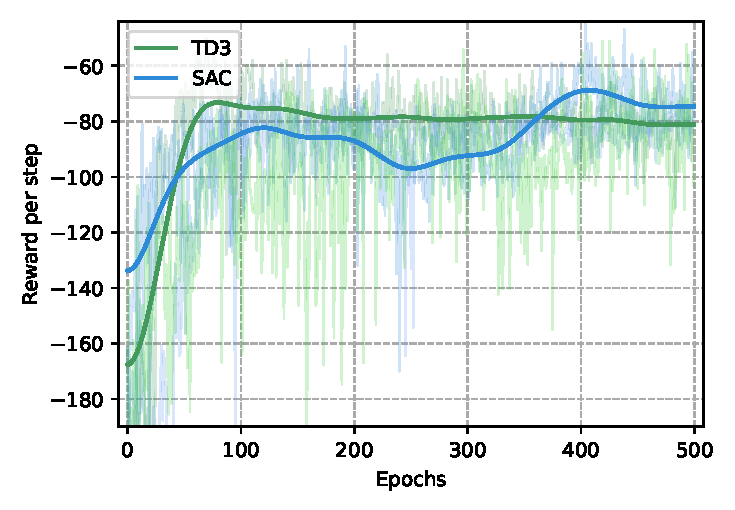
\includegraphics[width=0.502\linewidth]{TD3_SAC.pdf}
        \caption{Example training curves of SAC and TD3 algorithm under a same reward function.}
        \label{fig_1}
        \end{figure*}


The experiment utilizes the open-source implementation of the TD3\footnote{https://github.com/sfujim/TD3} algorithm \cite{2}, instead of the original paper's MAISAC, because SAC \cite{3} explores different requirements in multi-task learning. Although this approach improves the tolerance of the reward function and can achieve better results under suboptimal weight assignments, it also introduces greater randomness and fluctuations in the training results. Figure 2 illustrates this difference, and Table 2 lists the hyperparameters of the TD3 algorithm.






\section{Environment and Task Description} 

Task description is a common part of most subsequent prompts, comprising \verb|Env| class python code (or APIs), text description and numerical-explicit user requirements. 
 

\begin{minted}[breaklines,linenos,xleftmargin=20pt]{markdown}

## Task Overview

Key code of the environment in python are provided here, followed by a short description of the task.

```python
import numpy as np
from gym import spaces
class Env:
    def __init_(self, **kwargs):
        # --------------------
        #  Environment Parameters
        # --------------------
        self.N_POI = kwargs['NOO']  # Number of SNs, e.g. 50
        # Area position range (0,0) ~ (X_max,Y_max)
        self.X_max = kwargs['X_max'];
        self.Y_max = kwargs['Y_max']  # e.g. 120m
        self.border = np.array([self.X_max, self.Y_max])
        # Serving radius
        self.r_dc = kwargs['r_dc']  # e.g. 6m
        # Safe distance between AUVs
        self.safe_dist = kwargs['safe_dist']  # Safe distance between AUVs for avoiding collision, e.g. 8m
        # --------------------
        #  Variables
        # --------------------
        self.N_AUV = N  # Number of AUVs
        self.ec = np.zeros(self.N_AUV)  # Energy comsuption of AUVs
        self.SoPcenter = np.random.randint(10, self.X_max - 10, size=[self.N_POI, 2])  # Position of SNs
        self.target_Pcenter = np.zeros((self.N_UAV, 2))  # Position of target SNs (for AUV serving)
        self.Vxy = np.zeros(self.N_AUV, 2)  # x/y Velocity of AUVs
        self.xy = np.zeros((self.N_UAV, 2))  # Position of AUVs
        # --------------------
        # Some Metrics
        # --------------------
        self.crash = np.zeros(self.N_AUV, dtype=np.bool_)  # Collision between AUVs
        self.N_DO = 0  # Number of SNs data overflow (not served timely from AUVs)
        self.FX = np.zeros(self.N_AUV, dtype=np.bool_)  # Set to True when AUV crossing the border, else False
        self.TL = np.zeros(self.N_AUV,
                           dtype=np.bool_)  # Set to True when AUV successfully establish connection to the target SN, else False

    def compute_energy_consumption(self):  # Compute energy cosumption of AUVs
        V = np.linalg.norm(self.V, axis=1)
        S = 63;
        F = (0.7 * S * (V ** 2)) / 2
        self.ec = (F * V) / (-0.081 * (V ** 3) + 0.215 * (V ** 2) - 0.01 * V + 0.541)  # ~200W for 2m/s, ~70W for 1.3m/s

    def step(self, actions):  # A simplified pseudo-code for task executing
        # Actions contain velocity information of AUVs
        # actions.shape == (N_AUV,2) -> True
        for i in range(self.N_AUV):
            self.TL[i] = False;  # Same for self.crash/self.FX ...
            self.Vxy[:, 0] = (actions[0] * (self.max_speed)) * math.cos(actions[1] * math.pi)
            self.Vxy[:, 1] = (actions[0] * (self.max_speed)) * math.sin(actions[1] * math.pi)
            self.xy += self.Vxy
            # When distance constriant is met, AUV can establish the connection with the target SN
            if np.linalg.norm(self.xy[i] - self.target_Pcenter) <= self.r_dc:
                # Something TODO: hovering for data transmission, SN's replay buffer is cleared, ready for serving the next SN
                self.TL[i] = True
                pass
```

Description in Natural Language: `self.N_AUV` AUVs are deployed in an area measuring `self.border[0]` × `self.border[1]`. Each AUV must respond to data transfer requests from its corresponding target SN and navigate to the target device to prevent data overflow of SNs. After establishing a connection with an SN, the AUV will proceed to serve the next SN.

## Objectives of the task

Here are the main objectives to be optimized for the task: Safety requirements must be met first, followed by meeting performance requirements, and then optimizing energy consumption.

(Safety requirements) The number of both **collisions** and **border crossings** should be **reduced to zero**.

(Performance requirements) The number of data overflows **should be reduced to zero as much as possible**. This can be achieved by **responding promptly** to SNs and **increasing** the number of served SNs.

(Performance objective) The energy consumption of AUVs may be optimized (lower is better) without violating the **aforementioned** requirements.

\end{minted}

Since this description frequently appears in subsequent sections, it will be abbreviated as follows:

\begin{minted}[breaklines]{markdown}
===================
 <Env Description>
===================
\end{minted}

If this description is partially referenced, for instance, we denote the situation of referencing without a specific part as follows:

\begin{minted}[breaklines]{markdown}
==================================
 <Env Description w/o objectives>
==================================
\end{minted}


\section{Description Review Meta-Prompt (An example)} 

The description review meta-prompt instructs LLMs to critique prompts step by step and output them in a specific format to identify potential incompleteness and ambiguity. It should be noted that the prompt modification is still done manually and generally needs to be done only for the task description of custom environments. The following meta-prompt is input as the system message, and the user message takes the prompt used in Section 4.1 of this supplementary material (i.e., the reward code generator) as an example.

\subsection{Prompt}
\begin{minted}[breaklines,linenos,xleftmargin=20pt]{markdown}
You are an expert in prompt engineering. My goal is to obtain precise and effective responses for my code design task by providing GPT with specific and clear prompts. Following this, I'll provide some prompts. You should **not respond to the prompt's content in any way**. Instead, analyze the input prompt carefully. You should particularly consider the following issues:

- (Checklist item 1) Is the task description provided clear enough to represent the task? If not, where and in what form should additional information be provided?
- (Checklist item 2) Does the Python code provided lack necessary statements for understanding, conditions, and numerical references?
- (Checklist item 3) What suggestions do you have for improving the structure and organization of the prompt? Speculate on the intent of the prompt, identifying any scattered needs that the author should emphasize but that GPT might overlook in longer input prompts.
- (Checklist item 4) Does the prompt clearly and explicitly state the user’s needs? Are there any potential ambiguities in understanding?

In addition to these issues, you should identify problems in the prompt individually as much as possible. If necessary, quote parts of the prompt to further explain your points. Carefully analyze the prompt line by line from top to bottom if you encounter difficulties understanding it, and provide detailed modification suggestions and methods for each issue.

## Format for reference

### Clarity of Task Description (Checklist item 1)
**Issue 1 :**  Something...
**Suggestion1 :**  Something...
**Revision 1 :** Some specific rectified prompt snippets...
**Issue 2 :**  Something...
**Suggestion 2 :**  Something...
**Revision 2 :** Some specific rectified prompt snippets...
**Issue 3 :**  Something...
... (other issues, suggestions&revisions)

### Necessary Statements Inclusion  (Checklist item 2)
**Issue 1 :**  Something...
**Suggestion1 :**  Something...
**Revision 1 :** Some specific rectified prompt snippets...
**Issue 2 :**  Something...
**Suggestion 2 :**  Something...
**Revision 2 :** Some specific rectified prompt snippets...
**Issue 3 :**  Something...
... (other issues, suggestions&revisions)

### Structure & Organization  (Checklist item 3)
... (other issues, suggestions&revisions)

### Potential Ambiguities  (Checklist item 4)
... (other issues, suggestions&revisions)

### Other Issues
... (other issues, suggestions&revisions)
## Output Requirements

- **Do not output an integrated revised prompt.** Adhere to the previously mentioned format and provide quoted sections for revision along with suggestions. 
- All issues, suggestions, and revisions must refer to a specific part or paragraph of the given prompt and provide a revised example for each specific section. If there are issues with the prompt as a whole, you should point them out and utilize a section of the instruction to illustrate it, and present a corrected example.

\end{minted}
\subsection{Example Output}

\begin{minted}[breaklines,linenos,xleftmargin=20pt]{markdown}
### Clarity of Task Description (Checklist item 1)

**Issue 1:** The task description is fairly detailed, but the prompt could be more explicit about the specific reward structure requirements, such as the relative importance of each component (safety, performance, energy).

**Suggestion 1:** Clarify the priority order of the objectives, explicitly stating which components should be prioritized in the reward function.

**Revision 1:** 

```markdown
## Objectives Priority

The reward function should prioritize objectives in the following order:
1. Safety: Avoiding collisions and border crossings is the highest priority.
2. Performance: Reducing data overflow is the next priority.
3. Energy: Optimizing energy consumption is the least priority, only if it doesn't compromise the above objectives.
```

**Issue 2:** The prompt mentions "sparse and dense terms" but does not define these terms clearly for users unfamiliar with them.

**Suggestion 2:** Provide a brief explanation of what "sparse" and "dense" terms mean in the context of reinforcement learning reward functions.

**Revision 2:** 

```markdown

## Sparse vs. Dense Rewards

- **Sparse Rewards:** These are given only when specific events occur, like a collision or successfully connecting to a sensor node.
- **Dense Rewards:** These provide continuous feedback based on the current state, such as the distance to a target/obstacle or energy consumption.
```

### Necessary Statements Inclusion (Checklist item 2)

**Issue 1:** The code provided lacks initialization for some variables, such as `self.N_UAV`, which should likely be `self.N_AUV`.

**Suggestion 1:** Ensure all variables are correctly initialized and reference the correct names.

**Revision 1:** 

```python
# Correct initialization for number of AUVs
self.N_AUV = kwargs['N_AUV'] # number of AUVs
```

**Issue 2:** The `step` function references `self.V`, which is not initialized or defined in the provided code.

**Suggestion 2:** Ensure that all variables used in the methods are defined and initialized properly.

**Revision 2:** 

```python
# Correct velocity initialization
self.V = np.zeros((self.N_AUV, 2)) # Velocity of AUVs
```

### Structure & Organization (Checklist item 3)

**Issue 1:** The prompt could benefit from a more structured breakdown of each section, especially separating code from explanations.

**Suggestion 1:** Use headings and subheadings to clearly delineate sections like "Code Explanation," "Reward Function Requirements," and "Output Format."

**Revision 1:** 

```markdown
## Code Explanation

### Environment Setup
- Explanation of the environment parameters and initialization.

### Reward Function Requirements
- Detailed requirements for the reward function structure and priorities.

## Output Format
- Instructions on how to output the reward function code.
```

### Potential Ambiguities (Checklist item 4)

**Issue 1:** The prompt does not specify what should happen if there are conflicts between objectives, such as safety and energy consumption.

**Suggestion 1:** Explicitly state how to handle conflicts between objectives, emphasizing which should take precedence.

**Revision 1:** 

```markdown
## Conflict Resolution

In case of conflicts between objectives:
- Safety must always be prioritized over performance and energy consumption.
- Performance improvements should not compromise safety.
- Energy optimization is secondary to both safety and performance.
```

### Other Issues

**Issue 1:** The prompt does not specify the units or scales for some parameters, such as energy consumption or distances.

**Suggestion 1:** Provide units or scales for all measurable parameters to ensure consistency in calculations.

**Revision 1:** 

```markdown
## Parameters and Units

- Distances (e.g., `self.r_dc`, `self.safe_dist`) are measured in meters.
- Energy consumption (`self.ec`) is measured in watts.
- Velocity is measured in meters per second.
```

These revisions will help clarify the task, ensure the necessary information is included, and improve the structure and organization of the prompt for better comprehension and execution.

\end{minted}


\section{Reward Code Generator} 

The reward code generator provides a starting point for code search. We require that all code generation units align with user requirements (or a combination of two or more requirements), and the number of numerical values needed for adjustment not too much, without affecting the adjustment degrees of freedom. The prompt is provided in Section 4.1. At the same time, for certain tasks, the reward code generator can also incorporate human prior knowledge. For instance, we offers guidance for code generation to a certain extent and the corresponding output is in Section 4.3, compare to Section 4.2 with no guidance.

\subsection{Example prompt}

\begin{minted}[breaklines,linenos,xleftmargin=20pt]{markdown}

You are an expert in underwater information collection, reinforcement learning (RL), and reward function design. We will employ RL methods to complete the task of multiple AUVs collecting information from underwater sensor nodes (SNs). Here, instructions are provided in **Markdown** format; you should write a reasonable reward function to fulfill task requirements, and the reward function result should be formatted as a code block (Python code string of markdown `python ... `).

===================
 <Env Description>
===================

You should write each component by yourself. Try analyzing how to achieve the goal by finding the corresponding variables from the `Env` class, and produce the specific code to implement the sparse and dense terms of each user requirement, respectively.

## Output format

Considering that the generated code may need further human modifications, ensure that all reward coefficients or values requiring manual adjustments in the reward function are clearly defined separately from the core code content to avoid the presence of magic numbers, which are hard to adjust. Here is an example output, noting that it does not constitute any suggestions regarding the function content.

```python
def compute_reward(self):
    # ------ PARAMETERS  ------
    # parameters output independently
    w_ec;
    r_cs;
    # -------- Code ----------
    # Reward function core python code to be written
    reward += w_ec * ... # Utilizing parameter variables to calculate reward.
```

## Reward Function Requirements

- The function should strictly follow the format `def compute_reward(self)`, returning `reward`, an `np.ndarray` with shape `(self.N_AUV,)`.
- Ensure that your code follows the syntax rules of Python and contains no syntax errors. Additionally, only functions from the package `import numpy as np` are allowed to be used.
- The reward function should be defined in the `Env` class as `def compute_reward(self)`. It should only use variables within the class or create reasonable local variables.
- Under the premise of ensuring the necessary degrees of freedom, it is important to note that the number of parameters that need to be adjusted by the user (i.e., the number of variables defined in the PARAMETERS part) should be as small as possible. Generally speaking, the number should be approximately equal to or slightly exceed the number of user requirements.
- The reward function is expected to meet all previously demonstrated demands.
- Normalize all distance terms by dividing them by the area size (specifically, `np.linalg.norm(self.border)`).
- Before outputting the code, write an analysis, along with code snippets, on how to generate code for each user requirement.
- The code should be clear to read and easily modifiable. Add comments as you think necessary, like:

```python
# Thought: First, we can xxx, then xxx can be xxx...
# Penalty term: avoiding collision between AUVs
# the distance between AUVs 
# TODO: Here needs to be further improved
```

\end{minted}

We also try to provide some guides of generating reward components for each user requirement in the "objective of the task" section. The corresponding output is shown in Section 3.3. Corresponding complementary prompt is as follows:

\begin{minted}[breaklines,linenos,xleftmargin=20pt]{markdown}
- Avoiding collisions can be achieved by penalizing overly small distances between AUVs (dense reward) or the `self.crash[i]` term, which indicates a collision when `self.crash[i] == True` (sparse reward). 
- Avoiding crossing the border can be achieved by penalizing overly small distances between the AUV and the border (dense reward) or the `self.FX[i]` term, which indicates crossing the border (sparse reward). 
- Encouraging each AUV to serve target SNs promptly by rewarding the reduction in the distance between the i-th AUV and the target SN (dense reward) or the `self.TL[i]` term, which indicates successfully establishing a connection with the target SN. 
- Reducing energy consumption by penalizing `self.ec`.

\end{minted}

\subsection{Example Output}

\begin{minted}[breaklines,linenos,xleftmargin=20pt]{markdown}
## Analysis

To design the reward function for the task, we need to address three main objectives: safety, performance, and energy consumption. Here’s how we can break down each component:

### Safety Requirements

1. **Collision Avoidance**: We need to penalize any collisions between AUVs.
   - Use `self.crash` to identify collisions.
   - Add a large negative reward (`r_crash`) to penalize collisions.

2. **Boundary Crossing**: We need to penalize AUVs that cross the simulation boundary.
   - Use `self.FX` to check if any AUV has crossed the border.
   - Add a large negative reward (`r_border_cross`) to penalize boundary crossings.

### Performance Requirements

1. **Data Overflow Reduction**: We need to penalize the overflow of data in SNs.
   - Use `self.N_DO` to count the number of SNs that have overflowed.
   - Add a negative reward (`r_data_overflow`) for each overflow.

2. **Successful Connection**: We need to reward successful connections to SNs.
   - Use `self.TL` to check if an AUV has successfully connected to an SN.
   - Add a positive reward (`r_success_connect`) for each successful connection.

### Energy Consumption

1. **Energy Efficiency**: We need to minimize the energy consumption of AUVs.
   - Use `self.ec` to get the energy consumption of each AUV.
   - Add a negative reward (`w_energy * self.ec`) to penalize high energy consumption.

### Combining the Components

We will combine these components into a single reward function. The reward for each AUV will be the sum of the penalties and rewards from the above components, weighted appropriately.

### Parameters

We will define the parameters separately to make the reward function easily adjustable. The parameters will include weights for each component, and we will provide alternative values for these parameters.

### Code Snippets

Here is a breakdown of the code snippets for each component:

1. **Collision Avoidance**:
   ```python
   collision_penalty = np.where(self.crash, r_crash, 0)
   ```

2. **Boundary Crossing**:
   ```python
   border_cross_penalty = np.where(self.FX, r_border_cross, 0)
   ```

3. **Data Overflow Reduction**:
   ```python
   data_overflow_penalty = self.N_DO * r_data_overflow
   ```

4. **Successful Connection**:
   ```python
   success_connect_reward = np.where(self.TL, r_success_connect, 0)
   ```

5. **Energy Efficiency**:
   ```python
   energy_penalty = w_energy * self.ec
   ```

### Final Reward Function

Here is the complete reward function, combining all the components:

```python
def compute_reward(self):
    # ------ PARAMETERS ------
    w_energy;  # weight of energy consumption penalty
    r_crash;  # penalty for collision
    r_border_cross;  # penalty for crossing the border
    r_data_overflow;  # penalty for data overflow
    r_success_connect;  # reward for successful connection

    # -------- Code ----------
    # Collision penalty
    collision_penalty = np.where(self.crash, r_crash, 0)
    
    # Border crossing penalty
    border_cross_penalty = np.where(self.FX, r_border_cross, 0)
    
    # Data overflow penalty
    data_overflow_penalty = self.N_DO * r_data_overflow
    
    # Successful connection reward
    success_connect_reward = np.where(self.TL, r_success_connect, 0)
    
    # Energy consumption penalty
    energy_penalty = w_energy * self.ec
    
    # Total reward
    reward = collision_penalty + border_cross_penalty + data_overflow_penalty + success_connect_reward - energy_penalty
    
    return reward
```

This function adheres to the requirements and can be easily modified by adjusting the parameter values. The reward components are clearly separated and commented, making it straightforward to understand and tweak as needed.


\end{minted}

\subsection{Example Output (with prior knowledge for code generation)}

\begin{minted}[breaklines,linenos,xleftmargin=20pt]{markdown}
## Analysis

To create the reward function, we need to address the following key objectives:

1. **Safety Requirements:**
   - **Avoiding Collisions:** Penalize collisions between AUVs.
   - **Avoiding Border Crossing:** Penalize AUVs crossing the border.

2. **Performance Requirements:**
   - **Data Overflow:** Penalize data overflow.
   - **Timely Service:** Reward successful connections to SNs.

3. **Energy Consumption:**
   - **Optimize Energy Consumption:** Penalize high energy consumption.

### Steps to Implement the Reward Function

1. **Avoiding Collisions:**
   - **Sparse Reward:** Use `self.crash[i]` to penalize collisions.
   - **Dense Reward:** Penalize small distances between AUVs.

2. **Avoiding Border Crossing:**
   - **Sparse Reward:** Use `self.FX[i]` to penalize border crossings.
   - **Dense Reward:** Penalize small distances between AUVs and the border.

3. **Timely Service:**
   - **Sparse Reward:** Use `self.TL[i]` to reward successful connections.
   - **Dense Reward:** Reward decrease in distance between AUVs and their target SNs.

4. **Energy Consumption:**
   - Penalize the energy consumption of AUVs.

## Code Snippets for Each Component

- **Avoiding Collisions (Dense Reward):**
  ```python
  for i in range(self.N_AUV):
      for j in range(i+1, self.N_AUV):
          dist = np.linalg.norm(self.xy[i] - self.xy[j]) / np.linalg.norm(self.border)
          if dist < self.safe_dist / np.linalg.norm(self.border):
              reward[i] += w_collision * (dist - self.safe_dist / np.linalg.norm(self.border))
  ```

- **Avoiding Border Crossing (Dense Reward):**
  ```python
  for i in range(self.N_AUV):
      dist_to_border = np.min([self.xy[i][0], self.border[0] - self.xy[i][0], self.xy[i][1], self.border[1] - self.xy[i][1]]) / np.linalg.norm(self.border)
      if dist_to_border < self.safe_dist / np.linalg.norm(self.border):
          reward[i] += w_border * (dist_to_border - self.safe_dist / np.linalg.norm(self.border))
  ```

- **Timely Service (Dense Reward):**
  
  ```python
  for i in range(self.N_AUV):
      dist_to_target = np.linalg.norm(self.xy[i] - self.target_Pcenter[i]) / np.linalg.norm(self.border)
      reward[i] += w_service * (1 - dist_to_target)
  ```

## Full Reward Function

Here is the complete reward function code:

```python
def compute_reward(self):
    # ------ PARAMETERS  ------
    w_collision;  # weight for collision penalty
    w_border;  # weight for border crossing penalty
    w_service;  # weight for successful service reward
    w_overflow;  # weight for data overflow penalty
    w_energy;  # weight for energy consumption penalty
    
    # -------- Code ----------
    reward = np.zeros(self.N_AUV)
    
    # Penalty for collisions (sparse)
    for i in range(self.N_AUV):
        if self.crash[i]:
            reward[i] += w_collision
    
    # Penalty for border crossing (sparse)
    for i in range(self.N_AUV):
        if self.FX[i]:
            reward[i] += w_border
    
    # Reward for successful connection to SN (sparse)
    for i in range(self.N_AUV):
        if self.TL[i]:
            reward[i] += w_service
    
    # Penalty for data overflow (sparse)
    reward += w_overflow * self.N_DO
    
    # Penalty for energy consumption (dense)
    reward += w_energy * self.ec
    
    # Avoiding collisions (dense)
    for i in range(self.N_AUV):
        for j in range(i+1, self.N_AUV):
            dist = np.linalg.norm(self.xy[i] - self.xy[j]) / np.linalg.norm(self.border)
            if dist < self.safe_dist / np.linalg.norm(self.border):
                reward[i] += w_collision * (dist - self.safe_dist / np.linalg.norm(self.border))
    
    # Avoiding border crossing (dense)
    for i in range(self.N_AUV):
        dist_to_border = np.min([self.xy[i][0], self.border[0] - self.xy[i][0], self.xy[i][1], self.border[1] - self.xy[i][1]]) / np.linalg.norm(self.border)
        if dist_to_border < self.safe_dist / np.linalg.norm(self.border):
            reward[i] += w_border * (dist_to_border - self.safe_dist / np.linalg.norm(self.border))
    
    # Reward for timely service (dense)
    for i in range(self.N_AUV):
        dist_to_target = np.linalg.norm(self.xy[i] - self.target_Pcenter[i]) / np.linalg.norm(self.border)
        reward[i] += w_service * (1 - dist_to_target)
    
    return reward
```

This reward function should be integrated into the `Env` class and will help the AUVs to meet the task objectives by balancing safety, performance, and energy consumption.

\end{minted}

\section{Reward Critic} 

The reward critic follows instructions from a step-by-step guide, specifically by first listing possible reasons for code failure, then reviewing the environment code and the requirement, and finally outputting the correct function code. The requirements for rewriting code are the same as those for the reward code generator. Section 5.1 and 5.2 attempt to rectify the reward component that contains only sparse reward terms, while Section 5.3 rectifies an incorrect component, which inverts the punishment that should be given for a collision into a reward, reversing the symbol \verb|reward -= ...| to \verb|reward += ...|. These are the problems that actually arise when utilizing the reward code generator.

\subsection{Example Prompt of Inputting a Sparse Reward Component}

\begin{minted}[breaklines,linenos,xleftmargin=20pt]{markdown}
You are an expert in underwater information collection, reinforcement learning (RL), and reward component design. I am designing a reward component for completing an underwater information collection task, but the reward component is not componenting properly. You need to inspect the reward component to identify the issues. Then, analyze how to modify it effectively to align the reward component with the task requirements and guide the training strategy effectively.

==================================
 <Env Description w/o objectives>
==================================

## Objectives of the task

The user requirements I currently need to address are a subset of the task requirements, as indicated below.

(Safety requirements) The number of **collision** should **reduce to 0**.

However, this reward component fails to meet this requirement properly. 

```python
def compute_reward(self):
    # ------ PARAMETERS ------
    r_crash = -500  # penalty for collision
    # -------- Code ----------
    # Collision penalty
    collision_penalty = np.where(self.crash, r_crash, 0)
    reward = collision_penalty
    return reward
```

## Output the result step-by-step

- First, analyze the main reasons why the reward component fails to meet the user requirements. This could be due to the unreasonable format of the reward component, or it could be due to errors in the reward component. You should find them.
- Carefully analyze the environment code again to identify which variables, as part of the reward component, can guide the strategy to complete the task. Pay attention to breaking down the task requirements. A step-by-step analysis and listing of potential factors that could contribute, along with some snippets, may help in correctly analyzing the reasons.
- Output a revised and reasonable reward component.

Notice that you are only required to accomplish the user requirement subset mentioned before. DO NOT try to accomplish other requirements.

Considering that the generated code may need further human modifications, you must ensure that all reward coefficients or values requiring manual adjustments in the reward component are clearly defined separately from the core code content, to avoid the presence of magic numbers hard to adjust. Here a example showing the output format is given:

```python
def compute_reward(self):
    # ------ PARAMETERS  ------
    # The number of parameters that need to be adjusted by the user should be as small as possible, typically only one or two parameters are allowed
    # parameters output independently
    w_xx = 4;  # weight of xx
    r_xx = -200; # (sparse reward example)
    # -------- Code ----------
    # python code to be written
```

## Reward component Requirements

- The component should still follow the format `def compute_reward(self) `, return `reward`, an `np.ndarray` with shape `(self.N_AUV,)`.
- Ensure that your code follows syntax rules of python and contains no syntax errors. Besides, only components from the package `import numpy as np` are allowed to use.
- The reward component should be defined in the `Env` class as `def compute_reward(self)`. It should only use variables within the class or create reasonable local variables.
- Normalize all the distance terms by dividing all distances by the area size (namely `np.linalg.norm(self.border)`)
- The original reward component code contains numerical values. In your modified version, you should ensure that the numerical values of generated code are of the same order of magnitude. **Namely, it is not allowed to modify the original code only by the relevant coefficients.**
- The number of parameters that need to be adjusted by the user (i.e., the number of variables defined in the PARAMETERS part) should be as small as possible. Typically, only one or two parameters are allowed, and for the numerical that have no need to be adjusted by user, output it in the CODE part.
- If you think variables or functions in the code of task description is not enough to rewrite the reward component, you can fabricate these variables, but you should instruct user to complete them.
- The code is clear to read and easily modifiable. Add comment as you thought, like:

```python
# Thought: First, we can xxx, then xxx can be xxx...
# Penalty term: avoiding collision between AUVs
# the distance between AUVs 
# TODO: Here needs to be further improved
```


\end{minted}


\subsection{Example Output} 

\begin{minted}[breaklines,linenos,xleftmargin=20pt]{markdown}
To address the issue with the reward component for the underwater information collection task, we need to analyze why the current reward component fails to meet the requirement of reducing collisions to zero. Here’s a step-by-step breakdown of the analysis and the proposed solution:

### Step 1: Analyze the Main Reasons for Failure

1. **Sparse Reward Signal**: The current reward component only provides a penalty when a collision occurs (`r_crash = -500`). This is a very sparse reward signal, meaning that the agent only receives feedback when a collision happens. It doesn't guide the agent on how to avoid collisions proactively.

2. **Lack of Positive Reinforcement**: There is no positive reinforcement for maintaining safe distances or successfully navigating without collisions. The agent lacks an incentive structure that encourages safe behavior.

3. **No Consideration for Proximity**: The reward does not account for the proximity of AUVs to each other, which could help in guiding them to maintain safe distances.

### Step 2: Identify Variables to Guide Strategy

To effectively guide the strategy, the reward component should consider:

- **Proximity to Other AUVs**: Encourage AUVs to maintain a safe distance from each other.
- **Successful Connection Establishment**: While this is not directly related to the collision requirement, it can be useful to know that AUVs are reaching their targets without collisions.
- **Normalized Distance**: Incorporate the distance between AUVs, normalized by the area size, to provide a continuous signal that can help avoid collisions.

### Step 3: Revised Reward Component

Here is a revised reward component that addresses these issues:

```python
def compute_reward(self):
    # ------ PARAMETERS ------
    w_safe_dist = 10  # weight for maintaining a safe distance
    r_crash = -500  # penalty for collision
    safe_distance_threshold = self.safe_dist / np.linalg.norm(self.border)  # normalized safe distance
    # -------- Code ----------
    reward = np.zeros(self.N_AUV)

    # Penalty term: avoiding collision between AUVs
    collision_penalty = np.where(self.crash, r_crash, 0)
    reward += collision_penalty

    # Incentive for maintaining safe distances
    for i in range(self.N_AUV):
        for j in range(i + 1, self.N_AUV):
            distance = np.linalg.norm(self.xy[i] - self.xy[j]) / np.linalg.norm(self.border)
            if distance < safe_distance_threshold:
                # Penalize more as they get closer than the safe distance
                reward[i] -= w_safe_dist * (safe_distance_threshold - distance)
                reward[j] -= w_safe_dist * (safe_distance_threshold - distance)

    return reward
```

### Explanation of the Revised Reward Component

- **Collision Penalty**: The collision penalty remains the same, providing a strong negative signal when a collision occurs.

- **Safe Distance Incentive**: A new incentive is added for maintaining a safe distance between AUVs. If the distance between any two AUVs falls below the safe distance threshold, they are penalized. This penalty increases as they get closer, encouraging them to maintain safe distances.

- **Normalization**: All distance terms are normalized by the area size (`np.linalg.norm(self.border)`) to ensure consistency across different environment scales.

This revised reward component should provide a more continuous and informative signal to the learning agent, helping it to learn strategies that minimize collisions by maintaining safe distances between AUVs.

\end{minted}


\subsection{Full Version of Prompts and Answers in Fig. 2}

\subsubsection{Reward Critic - Prompt}

The prompt used in this part is consistent with Section 5.1, except the reward function is different:
 
 \begin{minted}[breaklines,linenos,xleftmargin=20pt]{python}
def compute_reward(self):
    # ------ PARAMETERS ------
    w_collision = -100  # weight for collision penalty
    # -------- Code ----------
    # Avoiding collisions (dense)
    for i in range(self.N_AUV):
        for j in range(i+1, self.N_AUV):
            dist = np.linalg.norm(self.xy[i] - self.xy[j]) / np.linalg.norm(self.border)
            if dist < self.safe_dist / np.linalg.norm(self.border):
                reward[i] += w_collision * (dist - self.safe_dist / np.linalg.norm(self.border))

\end{minted}

\subsubsection{Reward Critic - Output}

The modification claims in the original paper Fig. 2 appear in lines 46 and 47 of the text below, where you can see that the output component swaps the variables \verb|safe_dist_normalized| and \verb|dist|, so the final symbol of \verb|dist| is correct.

\begin{minted}[breaklines,linenos,xleftmargin=20pt]{markdown}
To address the issues with the reward component in your reinforcement learning environment for underwater information collection, let's go through a step-by-step analysis and provide a revised reward function that aligns with the task requirements, specifically focusing on reducing collisions to zero.

### Step-by-Step Analysis

1. **Current Reward Component Analysis:**

   - **Collision Penalty:** The current reward function penalizes collisions using a dense penalty scheme. It calculates the distance between every pair of AUVs and applies a penalty if the distance is below a safe threshold.
   
   - **Issues:**
     - The penalty is based on the difference between the current distance and the safe distance, which might not be effective enough to prevent collisions because the penalty might not be sufficiently large or immediate.
     - The reward calculation is not normalized properly, which could lead to scaling issues in larger environments.

2. **Environment Variables for Task Completion:**

   - **`self.xy`:** Positions of the AUVs, crucial for determining distances between AUVs.
   - **`self.safe_dist`:** The minimum safe distance to avoid collisions.
   - **`self.border`:** Used for normalizing distances to ensure consistent scaling across different environment sizes.

3. **Revised Reward Component Design:**

   - **Objective:** Enhance the collision penalty to ensure that AUVs maintain safe distances.
   - **Normalization:** Normalize distances by dividing by the area size (`np.linalg.norm(self.border)`).
   - **Penalty Structure:** Use a stronger penalty for collisions to ensure that the safety requirement is strictly enforced.

### Revised Reward Component

```python
def compute_reward(self):
    # ------ PARAMETERS ------
    w_collision = -100  # weight for collision penalty

    # -------- Code ----------
    # Initialize reward array
    reward = np.zeros(self.N_AUV)

    # Penalty term: avoiding collision between AUVs
    for i in range(self.N_AUV):
        for j in range(i + 1, self.N_AUV):
            # Calculate normalized distance between AUVs
            dist = np.linalg.norm(self.xy[i] - self.xy[j]) / np.linalg.norm(self.border)
            safe_dist_normalized = self.safe_dist / np.linalg.norm(self.border)
            
            # Apply penalty if AUVs are too close
            if dist < safe_dist_normalized:
                # Thought: Penalize more heavily as distance decreases below safe threshold
                reward[i] += w_collision * (safe_dist_normalized - dist)
                reward[j] += w_collision * (safe_dist_normalized - dist)

    return reward
```

### Explanation

- **Initialization:** The reward array is initialized for each AUV.
- **Distance Calculation:** The distance between each pair of AUVs is calculated and normalized by the environment size.
- **Collision Penalty:** A penalty is applied if the distance is less than the normalized safe distance. The penalty is proportional to how much the distance falls below the safe threshold, encouraging AUVs to maintain a safe separation.
- **Parameter Definition:** The penalty weight `w_collision` is defined separately for easy adjustment.

This revised reward component is designed to more effectively reduce the number of collisions to zero by applying a stronger and clearer penalty structure, ensuring that AUVs are incentivized to avoid getting too close to each other.
\end{minted}

\subsubsection{EUREKA-S - Prompt}

EUREKA-S modifies the reward function to include all required components. We hint in the prompt that there are errors in the EUREKA-S code and instruct EUREKA-S to rewrite the reward function. 


\begin{minted}[breaklines,linenos,xleftmargin=20pt]{markdown}
You are an expert in underwater information collection, reinforcement learning (RL), and reward function design. We have designed reward functions to complete underwater information collection tasks. **You need to find possible suggestions for improving the reward function code based on performance feedback, revising the function code, and rewrite a new reward function.**

===================
 <Env Description>
===================

## Reward function and log

The specific code for the reward function is as follows:

```python
    def compute_reward_(self):
        # -------- Code ----------
        reward = np.zeros(self.N_AUV)
        
        # Penalty for collisions (sparse)
        for i in range(self.N_AUV):
            if self.crash[i]:
                reward[i] -= 100
        
        # Penalty for border crossing (sparse)
        for i in range(self.N_AUV):
            if self.FX[i]:
                reward[i] -= 50
        
        # Reward for successful connection to SN (sparse)
        for i in range(self.N_AUV):
            if self.TL[i]:
                reward[i] += 100
        
        # Penalty for data overflow (sparse)
        reward -= 200 * self.N_DO
        
        # Penalty for energy consumption (dense)
        reward -= self.ec
        
        # Avoiding collisions (dense)
        for i in range(self.N_AUV):
            for j in range(i+1, self.N_AUV):
                dist = np.linalg.norm(self.xy[i] - self.xy[j]) / np.linalg.norm(self.border)
                if dist < self.safe_dist / np.linalg.norm(self.border):
                    reward[i] -= 100 * (dist - self.safe_dist / np.linalg.norm(self.border))
        
        # Avoiding border crossing (dense)
        for i in range(self.N_AUV):
            dist_to_border = np.min([self.xy[i][0], self.border[0] - self.xy[i][0], self.xy[i][1], self.border[1] - self.xy[i][1]]) / np.linalg.norm(self.border)
            if dist_to_border < self.safe_dist / np.linalg.norm(self.border):
                reward[i] -= 50 * (dist_to_border - self.safe_dist / np.linalg.norm(self.border))
        
        # Reward for timely service (dense)
        for i in range(self.N_AUV):
            dist_to_target = np.linalg.norm(self.xy[i] - self.target_Pcenter[i]) / np.linalg.norm(self.border)
            reward[i] += 100 * (1 - dist_to_target)
        
        return reward
```

**[Condensed log]**  
(num of collisions) [init]14.2 [init STD]18.9 [best]1.6 [final]27.8 [final STD]20.2

(num of crossing the border) [init]380.0 [init STD]80.1 [best]257.46 [final]264.12 [final STD]115.6

(num of data overflow) [init]7.07 [init STD]0.10 [best]6.67 [final]6.67 [final STD]0.302

(num of served SNs) [init]0.52 [init STD]0.5 [best]2.2 [final]2.2 [final STD]0.89

(energy consumption) [init]96.92 [init STD] 4.19 [best]65.22 [final]68.57 [final STD] 4.88

**[Summary]** The number of collisions shows a fluctuating trend and does not consistently reduce to 0, with the final value being 20.2. The number of border crossings remains high and fluctuates significantly, ending at 264.12, far from the required 0. Data overflows decrease slightly but remain high, concluding at 6.668, not meeting the requirement of reducing to 0. The number of served SNs improves, reaching 2.2, but with significant fluctuations. Energy consumption decreases significantly, ending at 68.566, closer to the theoretical minimum of 60W. 

## Output Guide

### A well-designed reward function has the following characteristics:
- The performance metrics 'data overflow', 'collision' and 'crossing the border' are expected to be as closed to 0 as possible. Accordingly, the number of the served SNs should be increased. **On the premise of meeting this**, the energy consumption should also be reduced.
- If the performance metrics are good, you should also pay attention to the stability of training, namely no significant fluctuations or high levels of STD in the metrics.

### To evaluate training performance, the following should be taken into account:
- Improvement in performance indicators compared to the beginning of training (i.e., random policy). 

- Whether the final achieved performance is close to the expected level. 

- Whether effective convergence is achieved after training, i.e., whether STD has significantly decreased compared to the initial stage, while the primary performance indicators have not shown significant changes.

### Here are some suggestions for reward function refinement:
- If all metrics do not show a significant increase as the training progresses, it implies that the reward function design is unreasonable. This may require a substantial re-scaling of the reward components to a proper range, or a reconstruction of some reward components (rewrite the reward component in another form, considering dense and sparse reward, and utilize other parameters in `Env` class, et.al). If the average reward increases but some performance metrics do not improve significantly or even decrease, it mean that the scale of the reward components needs to be adjusted to ensure a balance among multiple objectives. 

- When comparing between the reward functions, identifying groups of reward functions relatively perform well, extracting their advantages and eliminating their disadvantages. Finally, the designed reward function is expected to ensure **all metrics at a high level** simultaneously, while **minimizing fluctuations** after the training converges.

- You should look for errors in the code. **Output** whether there are errors and rectify them.

## Requirements

- The function should strictly follow the format `def compute_reward(self)`, returning `reward`, an `np.ndarray` with shape `(self.N_AUV,)`.
- Ensure that your code follows the syntax rules of Python and contains no syntax errors. Additionally, only functions from the package `import numpy as np` are allowed to be used.

- The reward function should be defined in the `Env` class as `def compute_reward(self)`. It should only use variables within the class or create reasonable local variables.

- The reward function is expected to meet all previously demonstrated demands.

- Normalize all distance terms by dividing them by the area size (specifically, `np.linalg.norm(self.border)`).

- The reward scale for each component should be balanced by adjusting the coefficients, and the total reward scale should be controlled between $10^1$ and $10^2$.
- The code should be clear to read and easily modifiable. Add comments as you think necessary, like:

```python
# Thought: First, we can xxx, then xxx can be xxx...
# Penalty term: avoiding collision between AUVs
# the distance between AUVs 
# TODO: Here needs to be further improved
```
\end{minted}

\subsubsection{EUREKA-S - Output}

From the output, we can see that EUREKA-S partially rewrites the reward function, but ultimately, the sign corresponding to the variable \verb|dist| is still negative, which indicates that EUREKA-S fails to correct the error.

\begin{minted}[breaklines,linenos,xleftmargin=20pt]{markdown}
To improve the reward function based on the given feedback and requirements, we need to address the performance metrics and ensure that they converge towards the desired values. The main issues with the current reward function are the fluctuations in performance metrics and the inability to reduce certain metrics to zero, such as collisions, border crossings and data overflow.

### Key Areas for Improvement:
1. **Collision and Border Crossing:** These should be heavily penalized to ensure safety requirements are met.
2. **Data Overflow:** Needs to be penalized more to encourage timely service of SNs.
3. **Energy Consumption:** Should be minimized but not at the expense of safety and performance requirements.
4. **Timely Service of SNs:** Should be rewarded to increase the number of served SNs.
5. **Normalization and Scaling:** Ensure all distance-related metrics are normalized and the reward components are scaled appropriately.

### Revised Reward Function

Here's a revised version of the reward function with detailed comments:

```python
def compute_reward(self):
    # Initialize reward array for each AUV
    reward = np.zeros(self.N_AUV)

    # Penalty for collisions (sparse)
    collision_penalty = -200
    for i in range(self.N_AUV):
        if self.crash[i]:
            reward[i] += collision_penalty

    # Penalty for border crossing (sparse)
    border_cross_penalty = -150
    for i in range(self.N_AUV):
        if self.FX[i]:
            reward[i] += border_cross_penalty

    # Reward for successful connection to SN (sparse)
    connection_reward = 150
    for i in range(self.N_AUV):
        if self.TL[i]:
            reward[i] += connection_reward

    # Penalty for data overflow (sparse)
    data_overflow_penalty = -250
    reward += data_overflow_penalty * self.N_DO

    # Penalty for energy consumption (dense)
    energy_penalty_factor = 0.1
    reward -= energy_penalty_factor * self.ec

    # Penalty for proximity to other AUVs (dense)
    collision_avoidance_penalty = 100
    for i in range(self.N_AUV):
        for j in range(i + 1, self.N_AUV):
            dist = np.linalg.norm(self.xy[i] - self.xy[j]) / np.linalg.norm(self.border)
            if dist < self.safe_dist / np.linalg.norm(self.border):
                reward[i] += collision_avoidance_penalty * (self.safe_dist / np.linalg.norm(self.border) - dist)

    # Penalty for proximity to border (dense)
    border_avoidance_penalty = 50
    for i in range(self.N_AUV):
        dist_to_border = np.min([self.xy[i][0], self.border[0] - self.xy[i][0], self.xy[i][1], self.border[1] - self.xy[i][1]]) / np.linalg.norm(self.border)
        if dist_to_border < self.safe_dist / np.linalg.norm(self.border):
            reward[i] += border_avoidance_penalty * (self.safe_dist / np.linalg.norm(self.border) - dist_to_border)

    # Reward for being closer to the target SN (dense)
    proximity_reward_factor = 50
    for i in range(self.N_AUV):
        dist_to_target = np.linalg.norm(self.xy[i] - self.target_Pcenter[i]) / np.linalg.norm(self.border)
        reward[i] += proximity_reward_factor * (1 - dist_to_target)

    return reward
```

### Explanation:
- **Collision and Border Crossing:** Increased penalties ensure these safety requirements are prioritized.
- **Data Overflow:** Increased penalty to strongly discourage allowing SNs to overflow.
- **Energy Consumption:** A smaller penalty factor encourages energy efficiency without compromising other objectives.
- **Proximity to Other AUVs and Borders:** Dense penalties encourage maintaining safe distances and staying within borders.
- **Timely Service:** Proximity rewards ensure AUVs are incentivized to reach SNs quickly, increasing the number of served SNs.

This revised reward function should help balance the various objectives and lead to improved and more stable performance across all metrics.
\end{minted}


\section{Prompts of Reward Weight Search} 
This section describes the second part of the ERFSL framework, the reward weight search process. Sections 6.1 and 6.2 provide prompts for the reward weight initializer. For Section 6.3 and subsequent sections, we adopt the weight groups and training results of the \textbf{500x off} experiment group from the original paper. Specifically, compared to the weight groups generated in Section 6.2, the energy penalty weight is increased by 50x, while the remaining weights are decreased to 1/10x compared to their original values. Sections 6.3 and 6.4 provide prompts for the training log analyzer. Section 6.5 provides prompts for two subprocesses of the reward weight searcher (adjustment suggestion generation and weight adjustment), as well as the baseline EUREKA-M for comparative experiments.

For all subsequent prompts, we use the reward function as follows:
\begin{minted}[breaklines,linenos,xleftmargin=20pt]{python}
def compute_reward(self): # defined in the Env class
        # ------ PARAMETERS  ------
        w_collision;
        w_border;
        w_service;
        w_overflow;
        w_energy;
        
        # -------- Code ----------
        reward = np.zeros(self.N_AUV)
        
        # Penalty for collisions (sparse)
        for i in range(self.N_AUV):
            if self.crash[i]:
                reward[i] += w_collision
        
        # Penalty for border crossing (sparse)
        for i in range(self.N_AUV):
            if self.FX[i]:
                reward[i] += w_border
        
        # Reward for successful connection to SN (sparse)
        for i in range(self.N_AUV):
            if self.TL[i]:
                reward[i] += w_service
        
        # Penalty for data overflow (sparse)
        reward += w_overflow * self.N_DO
        
        # Penalty for energy consumption (dense)
        reward += w_energy * self.ec
        
        # Avoiding collisions (dense)
        for i in range(self.N_AUV):
            for j in range(i+1, self.N_AUV):
                dist = np.linalg.norm(self.xy[i] - self.xy[j]) / np.linalg.norm(self.border)
                if dist < self.safe_dist / np.linalg.norm(self.border):
                    reward[i] -= w_collision * (dist - self.safe_dist / np.linalg.norm(self.border))
        
        # Avoiding border crossing (dense)
        for i in range(self.N_AUV):
            dist_to_border = np.min([self.xy[i][0], self.border[0] - self.xy[i][0], self.xy[i][1], self.border[1] - self.xy[i][1]]) / np.linalg.norm(self.border)
            if dist_to_border < self.safe_dist / np.linalg.norm(self.border):
                reward[i] -= w_border * (dist_to_border - self.safe_dist / np.linalg.norm(self.border))
        
        # Reward for timely service (dense)
        for i in range(self.N_AUV):
            dist_to_target = np.linalg.norm(self.xy[i] - self.target_Pcenter[i]) / np.linalg.norm(self.border)
            reward[i] += w_service * (1 - dist_to_target)
        
        return reward
\end{minted}

And we denote this reward function as:
\begin{minted}[breaklines]{markdown}
===================
 <Reward Function>
===================
\end{minted}




\subsection{Reward Weight Initializer - Prompt}

\begin{minted}[breaklines,linenos,xleftmargin=20pt]{markdown}
You are an expert in underwater information collection, reinforcement learning (RL), and reward function design. We are designing reward functions to utilize RL methods to complete the task of multiple AUVs in collecting information from underwater sensor nodes (SNs). This task involves multiple optimization objectives. However, it is important to ensure a balanced weighting of the reward components corresponding to these objectives. Now, you need to calculate the values of the reward components and generate possible values for **five(5)** sets of parameters based on these calculations.

===================
 <Env Description>
===================

## Task Guide

The code for the reward function is as follows:

===================
 <Reward Function>
===================

Now, complete the values of the corresponding weights in the form of a Python code block, following the format below:

```python
# ------ PARAMETERS  ------
w_collision = xxx; # some comments for choosing this value
w_border = xxx;
w_service = xxx;
w_overflow = xxx;
w_energy = xxx;
```

Here are guides for choosing the value for parameters:

- Ensure that the weighted sum of all reward components is approximately equal in magnitude and that they exhibit similar changes with respect to actions. To achieve this, you should output a preliminary calculation of the value of each reward component based on the given or custom example value. For reward components with conditional judgments (such as collision penalties), you can set a value that satisfies the penalty condition (for example: `dist = 5m`). Note the regularization term `/ np.linalg.norm(self.border)`. Finally, the weighted reward components should have the same scale.
- The returned reward values should be on the order of magnitude of $10^1$.

## Requirements

- You can only assign values to the given parameters and cannot add or remove any.
- The first set of parameters should be the one most likely to satisfy all user requirements. It should balance the weighted values of the reward components as much as possible. The remaining sets can involve scaling certain parameter values, with a minimum step size of 5x. Note that reducing the weight of some parameters means that the relative change in the remaining weights will increase, or vice versa. You should pay attention to the ratio changes between parameters and try to minimize the number of parameters adjusted.
- The weights for some components may be negative, thereby penalizing or rewarding certain behaviors, so ensure you do not get the signs wrong.

\end{minted}

\subsection{Reward Weight Initializer - Example Output}

\begin{minted}[breaklines,linenos,xleftmargin=20pt]{markdown}
To design a balanced reward function for the AUVs, we need to carefully choose the weights for each component of the reward function. The objective is to ensure that the weighted sum of all reward components is approximately equal in magnitude and that they exhibit similar changes with respect to actions.

Let's break down the reward components and calculate preliminary values based on example scenarios:

1. **Collision Penalty (`w_collision`)**: This is penalized when two AUVs are too close. Assume the penalty condition is met (e.g., `dist = 5m`), and calculate the penalty.

2. **Border Crossing Penalty (`w_border`)**: This is penalized when an AUV crosses the border. Assume the penalty condition is met (e.g., `dist_to_border = 5m`).

3. **Successful Service Reward (`w_service`)**: This is rewarded when an AUV successfully connects to a SN. Assume a full reward when the connection is established.

4. **Data Overflow Penalty (`w_overflow`)**: This is penalized based on the number of SNs not served in time.

5. **Energy Consumption Penalty (`w_energy`)**: This penalizes based on the energy consumed by AUVs, calculated in the `compute_energy_consumption` method.

### Preliminary Calculations

Let's assume the following example values for initial calculations:

- `np.linalg.norm(self.border) \approx 170` (for a 120x120 area)
- `dist = 5m` for collision and border crossing penalty conditions.

**Collision Penalty Example**:
- Penalty for each collision: `w_collision * (5 - 8) / 170 \approx -3 * w_collision / 170`

**Border Crossing Penalty Example**:
- Penalty for border crossing: `w_border * (5 - 8) / 170 \approx -3 * w_border / 170`

**Successful Service Reward Example**:
- Assume a full reward of `w_service` for each successful service.

**Data Overflow Penalty Example**:
- Assume `N_DO = 1`, penalty: `w_overflow * 1`

**Energy Consumption Example**:
- Assume energy consumption `ec \approx 200` for a fast-moving AUV.
- Penalty: `w_energy * 200`

### Weight Selection

The objective is to balance these components so that the resulting rewards are on the order of magnitude of \(10^1\). Here is a proposed set of weights that aim to achieve this balance:

```python
# ------ PARAMETERS  ------
w_collision = -50;  # Strong penalty for collisions
w_border = -50;     # Strong penalty for border crossing
w_service = 100;    # Reward for successful service
w_overflow = -30;   # Penalty for data overflow
w_energy = -0.1;    # Penalty for energy consumption
```

### Alternative Sets of Parameters

To explore different trade-offs, we can scale some of these parameters:

```python
# Set 2: Increase the penalty for collisions and border crossings
w_collision = -250;  # 5x increase
w_border = -250;     # 5x increase
w_service = 100;
w_overflow = -30;
w_energy = -0.1;

# Set 3: Increase the reward for successful service
w_collision = -50;
w_border = -50;
w_service = 500;     # 5x increase
w_overflow = -30;
w_energy = -0.1;

# Set 4: Increase the penalty for data overflow
w_collision = -50;
w_border = -50;
w_service = 100;
w_overflow = -150;   # 5x increase
w_energy = -0.1;

# Set 5: Increase the penalty for energy consumption
w_collision = -50;
w_border = -50;
w_service = 100;
w_overflow = -30;
w_energy = -0.5;     # 5x increase
```

These sets of parameters allow for exploring different priorities in the optimization objectives, such as prioritizing safety, performance, or energy efficiency. The first set is balanced, while the others emphasize specific aspects of the task.
\end{minted}

\subsection{Training Log Analyzer - Example Prompt}


We input Python-list style training logs are input into the training log analyzer. After every 30 episodes, the training logs record the mean and standard deviation of each performance metric. The training log analyzer is then tasked with outputting the performance summary of each input group, as well as the overall performance.

\begin{minted}[breaklines,linenos,xleftmargin=20pt]{markdown}
We provide training logs for several reward functions, taken from a data-collection reinforcement learning (RL) task. To guide the user in further tuning the parameters of the reward function, you need to write a summary for each log showing the key message, based on user requirements detailed below.

## User requirements

The main objectives to be optimized for the task are: 

(Safety requirements) The number of both **collision** and **crossing the border** should **reduce to 0**.

(Performance requirements) The number of data overflow **should reduce to 0 as possible**. By increasing the number of served SNs, data overflow can be restrained.

(Performance objective) The energy consumption of AUVs may be optimized (lower is better) without violating the two requirements before. The value of energy consumption is between 60W and 170W.

## Output guide

There are multiple sets of weight parameters and the performance training logs that are generated by training policies using these weight parameters. You should first consider summarizing each group of performance results individually, and then compare them with each other.

For each group of inputs, you should first output a detailed analysis of performance separately, including a target value of a certain performance metric (such as converging to 0), an initial value (indicating the performance of a random policy), the trend of changes, and the trend of fluctuations (standard deviation). Subsequently, you should compress the above analysis. Here are possible examples for summarizing:


Output log:

```
AVG num of collisions:[287.583, 110.833, 29.667, 1.417, 2.25, 11.833, 0.0, 5.75, 3.5, 0.0]
AVG num of crossing the border:[950.125, 199.792, 256.917, 52.125, 112.417, 142.625, 54.375, 78.0, 97.167, 171.208]
```

Preliminary output: According to the training log, the number of collisions decreases gradually from an initial high value exceeding 200 to zero as training progresses. The data has decreased steadily, meeting user requirements. However, the number of boundary crossings, although decreasing during training, still remains around 100 at the conclusion, exhibiting significant fluctuations, which clearly deviates from the user requirement of zero occurrences.

Summarized output: Collision occurrences have significantly reduced to zero as training progresses, but occasional boundary crossings still persist with some fluctuations.

Full example: Collision occurrences have significantly reduced to zero as training progresses, but occasional boundary crossings still persist with some fluctuations. While the number of served SNs has seen an increase; however, it has subsequently remained at a very low level. Therefore, the number of overflows decreased to one-third of the initial value, but it still does not meet the requirements. Energy consumption, after optimization, has ultimately settled near the minimum value.


Next, one should consider which weight coefficients were adjusted for various input groups and how these adjustments influenced the training trends. It is important to note that training trends may sometimes vary significantly (noticeable to the user) while at other times they may not. Here is an example; please note that these examples are provided solely for formatting constraints and do not constitute content suggestions. Please follow the provided format, retaining the content within parentheses verbatim, and ensure to provide detailed corresponding analyses that reference performance metrics, user requirements, weight variables, numerical values, and other relevant factors.

## Format Example

(Summarizing the first group) The performance pertaining to safety requirements of input group 1 did not exhibit any improvement during training, remaining far from meeting user requirements. The SN service demonstrated some improvement; however, the number of data overflows decreased to only half of the initial value, still failing to meet user requirements, whereas energy consumption approached the theoretical minimum. (Difference between the second group and subsequent groups from the first group) Input group 2 increased the weight of the SN service `w_service` by five times, significantly reducing the number of overflows to a minimal level, thereby demonstrating considerable performance improvement, despite a slight degradation in energy consumption. Input group 3 increased the penalty weight for collision avoidance `w_collision` by five times; however, the overall performance improvement was minimal.[subsequent 3 groups] (Overall summary) Overall, the increase in the weight of the SN service in input group 2 had a significant effect, whereas the final effects of the other attempts remained unchanged.

Another abridged example: The performance concerning safety requirements of input group 1 exhibited no improvement during training, significantly failing to meet user requirements. The number of served SNs reached approximately 2 by the end, with virtually no observable decrease in the number of data overflows, while energy consumption approached the theoretical minimum. Despite adjustments to various weights in input groups 2, 3, and 4, the overall effects achieved were minimal, bordering on negligible. Overall, all groups demonstrated relatively efficient performance in terms of energy consumption; however, they fell short in meeting other requirements.

## Tips and requirements

- Attention should also be paid to trends that are often overlooked when summarizing. For instance, an indicator may still exhibit significant fluctuations in its average value or have a high standard deviation in the latter part of training. In the context of multi-task optimization, an increase in one performance indicator might be accompanied by a decrease in another or several other indicators, or vice versa.
- It is important to refer to the initial values of training and compare them to the reference values mentioned in the user requirements to summarize the performance indicators. For example, the number of data overflows should be reduced to zero whenever possible. Some examples for generating the answer include: (a) the number of overflows decreased to one-third of the initial value but still does not meet the requirements; (b) the power consumption eventually dropped to 70W, which is very close to the theoretical minimum.

## Performance result

Here is the performance log you need to analyze, [HGH] means higher is better, while [LOW] means lower is better.

### Group 1

```python
# ------ WEIGHTS  ------
w_collision = -5;  # Strong penalty for collisions
w_border = -5;     # Strong penalty for border crossing
w_service = 10;    # Reward for successful service
w_overflow = -3;   # Penalty for data overflow
w_energy = -5;    # Penalty for energy consumption
```

[HGH]AVG of total served SNs: [0.52, 0.92, 1.04, 0.68, 0.76, 0.68, 1.16, 1.2, 2.2, 2.36, 1.32, 0.16, 0.28, 0.68]
[LOW]STD of total served SNs: [0.5, 1.197, 1.038, 1.048, 0.907, 0.926, 1.567, 1.497, 1.327, 1.439, 1.462, 0.543, 0.531, 0.882]
[LOW]AVG num of data overflow: [7.082, 6.894, 6.869, 7.012, 7.042, 7.048, 6.887, 6.92, 6.701, 6.629, 6.953, 7.14, 7.105, 7.012]
[LOW]STD num of data overflow: [0.111, 0.501, 0.338, 0.257, 0.216, 0.155, 0.527, 0.422, 0.425, 0.438, 0.306, 0.107, 0.148, 0.242]
[LOW]AVG num of collisions: [5.28, 2.76, 5.92, 9.4, 14.36, 7.92, 11.2, 7.08, 13.2, 0.2, 20.52, 15.84, 2.4, 3.44]
[LOW]STD num of collisions: [25.867, 7.706, 22.043, 27.768, 31.356, 16.728, 33.211, 21.804, 32.056, 0.98, 49.684, 28.394, 6.35, 9.896]
[LOW]AVG num of crossing the border: [376.98, 59.02, 81.36, 130.42, 125.4, 106.48, 195.7, 177.72, 97.96, 105.88, 239.38, 163.8, 68.62, 183.9]
[LOW]STD num of crossing the border: [82.896, 58.945, 76.676, 153.036, 151.032, 96.039, 155.72, 116.317, 82.285, 141.463, 114.009, 163.214, 88.349, 169.732]
[LOW]AVG of energy consumption: [97.261, 77.054, 59.615, 57.99, 57.786, 56.786, 61.192, 60.407, 56.72, 57.125, 63.258, 59.355, 54.905, 60.58]
[LOW]STD of energy consumption: [4.407, 8.556, 3.537, 7.229, 7.294, 4.769, 7.61, 5.47, 4.005, 6.586, 5.515, 7.866, 4.29, 8.008]

### Group 2

```python
# Set 2: Increase the penalty for collisions and border crossings
w_collision = -25;  # 5x increase
w_border = -25;     # 5x increase
w_service = 10;
w_overflow = -3;
w_energy = -5;
```


[HGH]AVG of total served SNs: [0.48, 0.08, 0.36, 0.4, 0.24, 0.24, 1.04, 1.92, 2.08, 1.36, 0.48, 1.88, 0.92, 1.88]
[LOW]STD of total served SNs: [0.5, 0.271, 0.686, 0.566, 0.585, 0.512, 1.148, 1.017, 1.017, 1.162, 0.854, 0.909, 0.744, 1.143]
[LOW]AVG num of data overflow: [7.088, 7.169, 7.11, 7.109, 7.141, 7.145, 6.952, 6.692, 6.571, 6.788, 7.015, 6.806, 7.048, 6.881]
[LOW]STD num of data overflow: [0.101, 0.076, 0.196, 0.102, 0.16, 0.09, 0.238, 0.345, 0.409, 0.394, 0.256, 0.303, 0.138, 0.283]
[LOW]AVG num of collisions: [0.0, 19.2, 5.96, 20.96, 9.88, 2.08, 2.44, 3.56, 9.16, 6.08, 0.0, 1.08, 1.6, 4.2]
[LOW]STD num of collisions: [0.0, 32.002, 11.595, 75.631, 18.1, 9.002, 6.171, 17.037, 43.666, 15.242, 0.0, 2.544, 6.717, 15.448]
[LOW]AVG num of crossing the border: [378.58, 55.3, 79.44, 60.08, 207.12, 137.04, 91.72, 398.68, 342.8, 215.4, 204.58, 108.3, 96.34, 212.16]
[LOW]STD num of crossing the border: [78.581, 52.882, 74.584, 129.553, 131.189, 82.139, 79.873, 70.87, 123.934, 118.767, 114.545, 140.521, 73.382, 115.441]
[LOW]AVG of energy consumption: [96.251, 76.672, 59.178, 54.546, 61.557, 58.18, 56.197, 71.138, 68.598, 62.26, 61.476, 57.14, 56.252, 62.021]
[LOW]STD of energy consumption: [3.068, 8.903, 4.515, 6.189, 6.244, 3.915, 3.761, 3.477, 6.005, 5.637, 5.519, 6.702, 3.441, 5.576]

### Group 3

```python
w_collision = -5;
w_border = -5;
w_service = 50;     # 5x increase
w_overflow = -3;
w_energy = -5;
```

[HGH]AVG of total served SNs: [0.52, 0.04, 0.48, 2.4, 2.08, 0.96, 1.6, 0.96, 1.04, 0.84, 0.52, 1.08, 2.04, 2.88]
[LOW]STD of total served SNs: [0.5, 0.196, 0.574, 1.497, 1.719, 1.148, 1.356, 0.196, 1.216, 1.155, 0.755, 0.891, 1.536, 2.658]
[LOW]AVG num of data overflow: [7.09, 7.162, 7.083, 6.504, 6.704, 6.967, 6.809, 7.073, 6.986, 7.015, 7.05, 6.957, 6.678, 5.866]
[LOW]STD num of data overflow: [0.103, 0.057, 0.164, 0.441, 0.442, 0.274, 0.414, 0.047, 0.302, 0.274, 0.195, 0.246, 0.365, 0.745]
[LOW]AVG num of collisions: [8.36, 24.72, 1.96, 0.92, 0.56, 7.84, 0.84, 2.52, 7.32, 4.12, 4.64, 0.44, 0.96, 1.16]
[LOW]STD num of collisions: [18.317, 41.542, 4.152, 3.298, 2.368, 21.49, 3.916, 4.527, 20.224, 13.021, 17.486, 1.791, 2.793, 3.196]
[LOW]AVG num of crossing the border: [380.96, 52.1, 7.36, 23.8, 13.32, 120.64, 125.36, 42.4, 216.72, 143.6, 85.54, 85.78, 67.78, 42.1]
[LOW]STD num of crossing the border: [82.466, 45.539, 18.483, 50.931, 29.259, 100.173, 148.53, 38.722, 148.54, 99.713, 98.323, 72.813, 75.733, 57.322]
[LOW]AVG of energy consumption: [96.957, 76.588, 56.087, 53.268, 52.556, 57.549, 57.911, 53.582, 62.094, 58.628, 55.755, 55.985, 55.302, 54.883]
[LOW]STD of energy consumption: [3.429, 8.702, 2.568, 2.591, 1.462, 4.969, 7.021, 1.874, 7.098, 4.822, 4.721, 3.437, 3.482, 2.94]


### Group 4

```python
w_collision = -5;
w_border = -5;
w_service = 10;
w_overflow = -15;   # 5x increase
w_energy = -5;
```

[HGH]AVG of total served SNs: [0.56, 0.96, 0.64, 1.0, 1.88, 1.24, 1.64, 1.2, 0.76, 1.2, 0.32, 1.12, 1.04, 0.48]
[LOW]STD of total served SNs: [0.496, 1.28, 0.742, 1.131, 1.275, 0.709, 1.054, 0.693, 1.031, 1.166, 0.786, 1.032, 0.824, 0.7]
[LOW]AVG num of data overflow: [7.075, 6.939, 7.025, 6.954, 6.652, 6.961, 6.824, 6.999, 7.012, 6.905, 7.081, 6.941, 6.912, 7.031]
[LOW]STD num of data overflow: [0.123, 0.327, 0.221, 0.275, 0.464, 0.267, 0.342, 0.146, 0.3, 0.28, 0.265, 0.288, 0.271, 0.254]
[LOW]AVG num of collisions: [1.88, 10.56, 6.96, 8.88, 0.56, 11.48, 1.8, 1.48, 2.08, 4.0, 3.36, 1.2, 8.6, 22.8]
[LOW]STD num of collisions: [7.901, 22.872, 15.379, 22.288, 2.08, 35.005, 8.04, 3.113, 4.939, 12.007, 6.91, 2.298, 25.963, 36.23]
[LOW]AVG num of crossing the border: [380.88, 76.16, 142.34, 231.36, 234.08, 200.38, 60.08, 78.14, 131.66, 141.54, 99.24, 80.68, 111.4, 62.14]
[LOW]STD num of crossing the border: [91.573, 57.659, 93.922, 155.75, 168.526, 99.651, 66.369, 72.347, 158.411, 84.455, 90.745, 119.202, 119.065, 60.29]
[LOW]AVG of energy consumption: [97.512, 77.876, 62.121, 62.903, 63.329, 61.399, 55.005, 55.433, 58.113, 58.713, 56.379, 55.684, 57.202, 54.626]
[LOW]STD of energy consumption: [4.427, 8.401, 4.451, 7.451, 7.922, 4.811, 3.278, 3.544, 7.63, 4.191, 4.489, 5.771, 5.747, 2.891]

### Group 5

```python
w_collision = -5;
w_border = -5;
w_service = 10;
w_overflow = -3;
w_energy = -20;    # 4x increase
```

[HGH]AVG of total served SNs: [0.6, 0.08, 0.48, 0.48, 0.44, 0.52, 0.56, 0.32, 1.32, 0.12, 0.0, 0.0, 0.04, 0.8]
[LOW]STD of total served SNs: [0.49, 0.271, 0.7, 0.574, 0.571, 0.854, 0.496, 0.676, 0.926, 0.325, 0.0, 0.0, 0.196, 0.8]
[LOW]AVG num of data overflow: [7.054, 7.171, 7.035, 7.092, 7.124, 7.014, 7.061, 7.116, 6.908, 7.144, 7.186, 7.181, 7.173, 6.931]
[LOW]STD num of data overflow: [0.095, 0.068, 0.254, 0.175, 0.085, 0.208, 0.167, 0.202, 0.239, 0.116, 0.043, 0.039, 0.06, 0.26]
[LOW]AVG num of collisions: [12.0, 13.52, 13.84, 5.44, 0.0, 0.0, 7.16, 25.76, 9.48, 51.16, 5.96, 28.04, 21.52, 85.88]
[LOW]STD num of collisions: [51.582, 29.492, 22.159, 17.729, 0.0, 0.0, 13.925, 45.566, 16.909, 81.952, 10.486, 51.603, 32.894, 100.452]
[LOW]AVG num of crossing the border: [380.4, 103.7, 31.3, 62.08, 48.12, 13.56, 131.62, 64.46, 88.68, 202.9, 82.52, 74.62, 160.48, 97.16]
[LOW]STD num of crossing the border: [79.712, 81.144, 49.065, 80.312, 107.924, 28.619, 100.345, 60.227, 112.982, 127.159, 93.471, 103.435, 116.266, 119.157]
[LOW]AVG of energy consumption: [97.09, 77.447, 57.242, 54.637, 53.958, 52.283, 57.943, 54.727, 56.037, 61.245, 55.414, 55.05, 59.222, 56.433]
[LOW]STD of energy consumption: [4.323, 8.082, 3.449, 3.889, 5.211, 1.458, 4.736, 2.936, 5.434, 6.159, 4.479, 4.968, 5.619, 5.787]
\end{minted}


\subsection{Training Log Analyzer - Example Output}

\begin{minted}[breaklines,linenos,xleftmargin=20pt]{markdown}
Certainly! Let's analyze and summarize the performance of each group based on the training logs provided, focusing on the key objectives and adjustments in weight parameters.

### Group 1

**Detailed Analysis:**
- **Collisions:** Initial average of 5.28, fluctuating significantly throughout training, peaking at 20.52, and ending with a high fluctuation, indicating inconsistency and not meeting safety requirements.
- **Crossing the Border:** Starts at a high 376.98, decreases initially but ends around 183.9, with high fluctuations throughout, not meeting safety requirements.
- **Data Overflow:** Remains fairly constant around 7, with slight fluctuations, not approaching the target of 0.
- **Energy Consumption:** Decreases from 97.261 to around 60, showing improvement but with fluctuations.

**Summarized Output:** Collision occurrences fluctuate significantly without consistent reduction, and boundary crossings remain high, both not meeting safety requirements. Data overflow remains constant, not meeting performance requirements, while energy consumption improves but fluctuates.

### Group 2

**Detailed Analysis:**
- **Collisions:** Initial average of 0, spikes to 20.96, fluctuates widely, indicating instability and not meeting safety requirements.
- **Crossing the Border:** Starts at 378.58, decreases but fluctuates widely, ending high, not meeting safety requirements.
- **Data Overflow:** Remains around 7, with slight fluctuations, not meeting performance requirements.
- **Energy Consumption:** Decreases from 96.251 to around 62, showing improvement but with fluctuations.

**Summarized Output:** Despite increased penalties, collision and boundary crossing occurrences fluctuate widely, not meeting safety requirements. Data overflow remains unchanged, and energy consumption improves but with fluctuations.

### Group 3

**Detailed Analysis:**
- **Collisions:** Starts at 8.36, decreases to around 1.16, showing improvement but still with fluctuations.
- **Crossing the Border:** Decreases significantly from 380.96 to 42.1, showing improvement but still fluctuating.
- **Data Overflow:** Decreases slightly to 5.866, showing some improvement but not meeting the target.
- **Energy Consumption:** Decreases to around 54.883, with reduced fluctuations, showing good optimization.

**Summarized Output:** Collisions and boundary crossings decrease but still fluctuate, not fully meeting safety requirements. Data overflow shows slight improvement. Energy consumption is optimized well.

### Group 4

**Detailed Analysis:**
- **Collisions:** Starts at 1.88, fluctuates widely, peaking at 22.8, not meeting safety requirements.
- **Crossing the Border:** Starts high at 380.88, fluctuates and ends at 62.14, not meeting safety requirements.
- **Data Overflow:** Remains around 7, with slight fluctuations, not meeting performance requirements.
- **Energy Consumption:** Decreases to 54.626, showing good optimization with reduced fluctuations.

**Summarized Output:** Collisions and boundary crossings remain high with fluctuations, not meeting safety requirements. Data overflow remains unchanged. Energy consumption is optimized well.

### Group 5

**Detailed Analysis:**
- **Collisions:** Starts at 12, fluctuates widely, peaking at 85.88, not meeting safety requirements.
- **Crossing the Border:** Starts at 380.4, decreases but fluctuates widely, not meeting safety requirements.
- **Data Overflow:** Remains around 7, with slight fluctuations, not meeting performance requirements.
- **Energy Consumption:** Decreases to around 56.433, showing improvement but with fluctuations.

**Summarized Output:** Collisions and boundary crossings fluctuate widely without consistent reduction, not meeting safety requirements. Data overflow remains unchanged, and energy consumption improves but fluctuates.

### Overall Summary

The adjustments in weight parameters across all groups did not lead to consistent improvements in safety and performance requirements. Group 3 showed some promise with a decrease in collisions and boundary crossings, but fluctuations persisted. Energy consumption was generally optimized across groups, but safety and data overflow requirements were not met consistently. Further tuning of weight parameters, particularly focusing on stabilizing safety metrics, is necessary.

\end{minted}


\subsection{Reward Weight Searcher} 

We input the weight groups and the corresponding performance summaries in the following format:

\begin{minted}[breaklines,linenos,xleftmargin=20pt]{markdown}
### Group 1

```python
# ------ WEIGHTS  ------
w_collision = ...
...
```

[condensed training logs]
(num of collisions) [init]5.28 [init STD]25.87 [best]0.2 [final]3.44 [final STD]9.9
(num of crossing the border) [init]376.98 [init STD]82.9 [best]59.02 [final]183.9 [final STD]169.73
(num of data overflow) [init]7.08 [init STD]0.11 [best]6.63 [final]7.01 [final STD]0.24
(num of served SNs) [init]0.52 [init STD]0.5 [best]2.36 [final]0.68 [final STD]0.88
(energy consumption) [init]97.26 [init STD]4.41 [best]54.9 [final]60.58 [final STD]8.01

**Summarized Output:** Collision occurrences fluctuate significantly without consistent reduction... (same as those in Section 6.4)

### Group 2
...

### Overall Summary

The adjustments in weight parameters across all groups did not lead to consistent improvements in safety and performance requirements...

\end{minted}

And then denote them as:

\begin{minted}[breaklines]{markdown}
===========================================
 <Input Weight Groups & TLA Perf. Summary>
===========================================
\end{minted}

The prompt of reward weight searcher is divided into two sub-prompts: adjustment suggestion generation and weight adjustment, with the corresponding prompts detailed in Sections 6.5.1 and 6.5.3, respectively. Again, the examples provided are based on the training results of the \textbf{500x off} experiment group, and the weight groups are consistent with those in Section 6.3.

\subsubsection{Adjustment Suggestion Generation (Subprocess 1) - Example Prompt} 

The first subprocess generates textual modification suggestions based on the context provided by the training log analyzer, while deferring the actual output of weight groups to the second subprocess. In the first subprocess, we task LLMs to adjust each weight by specifying the starting point of the input group and the necessary step size. We refer to this process as mutation, borrowing from genetic algorithm terminology, but our "mutation" process is both active and directed. The purpose of the "mutation" process is to address the issue that, for multiple input groups, if the starting point is not specified, LLMs adjust the weights based on the first group by default. However, subsequent groups may already be adjusted based on the input group, potentially leading to redundant changes in the output group. Refer to the example in the prompt: if these two weight groups are inputted:

\begin{minted}[breaklines,linenos,xleftmargin=20pt]{markdown}

### Input Group 1

```python
# -------- PARAMETERS --------
    w_a = 3; # weight of requirement A
    w_b = 3; # weight of requirement B
    w_another = 2;
```
### Input Group 2

```python
# -------- PARAMETERS --------
    w_a = 15; # 5x increase
    w_b = 3;
    w_another = 2;
```
\end{minted}

And if the conclusion is that the weight of requirement A may increase 5x, LLMs will directly adjust the variable \verb|w_a| based on input group 1 (the default starting point) if the adjustment starting point is not specified, leading to duplication in input group 2:

\begin{minted}[breaklines,linenos,xleftmargin=20pt]{markdown}

### Output Group: increase the weight of `w_a`

```python
# -------- PARAMETERS --------
    w_a = 15; # 5x increase
    w_b = 3;
    w_another = 2;
```
\end{minted}

Additionally, to eliminate ambiguity in the adjustments, we task LLMs with reducing the number of adjustment parameters. Finally, some proposed suggestions adjust only a single weight, while others adjust multiple weights. In such cases, we integrate the accumulated adjustments of two or more mutated (adjusted) input groups relative to the starting point. We term this process "crossover". This process ensures the diversity of output group attempts, thereby increasing targeting and search scope.





\begin{minted}[breaklines,linenos,xleftmargin=20pt]{markdown}
You are an expert in underwater information collection, reinforcement learning (RL), and reward function design. We have designed reward functions to complete underwater information collection tasks. However, since these reward functions need to satisfy multiple user requirements, the weight parameters for these requirements may not be designed reasonably, and therefore it may not be possible to satisfy all requirements. Now, based on the given reward functions, reward and weight coefficients, and performance logs, you need to provide **five(5)** suggestions for modifying the weight coefficients.

===================
 <Env Description>
===================

## Reward function, weights and logs

The specific code for the reward function is as follows:

===================
 <Reward Function>
===================

The weight coefficients and their corresponding performance results are given below:

===========================================
 <Input Weight Groups & TLA Perf. Summary>
===========================================

## Output Guide

Due to multiple input sets, it is necessary to inspect the performance changes resulting from variations in the weights, adjusting the weight values to achieve user goals as quickly as possible while ensuring a broad exploration range.

- **Weight adjustment and performance analysis**: The first input group is the starting point for the search, with all other input groups adjusted based on the first group. You need to output which weight variables corresponding to specific user requirement(s) the second and subsequent input groups have changed relative to the first set. Following this, analyze the impact of these adjustments on performance in term of direction and degree, both from the performance summarization and by directly referencing performance metrics (favoring the latter in case of conflicts).  Also, explain what these changes in metrics signify. Additionally, explain the characteristics in common of these input groups.

- **Listing possible reasons & Proposing solutions**: Analyze why the input groups may fail to meet user requirements. This may be caused by either relatively small weight values directly corresponding to certain requirement(s) or some requirement(s) being overly optimized. You need to analyze how to adjust each weight to better meet user needs. Firstly, analyze the direction in which a weight should be adjusted if necessary, increasing or decreasing the weight further when some requirements are not met. For fine-tuning adjustments, you can opt for intermediate weight values (as there are more than one weight value corresponding to an input) or maintain the weight at the starting point value, or align it with search strategy that a input group have already been performed. Additionally, analyze adjustment strategies, including cases where only one weight needs adjustment or when more than one weight requires adjustment, combining the adjusting strategies for these weights, following the principles presented below. Considering the principle of minimum weight adjustment, the number of weights modified relative to the starting point should generally be kept below half (in this case, no more than two weights) for each search group.

- **Adjustment step size**: The step size should increase to ensure a broad enough exploration range, or decrease to make refined search when necessary. Typically, larger step sizes such as 5x, 10x (or 1/5x, 1/10x for decreasing) and smaller step sizes like 1.5x, 2x (or 1/1.5x, 1/2x for decreasing) are common principles to follow. Some examples for determining the basic step size:
  -  When inputs are `w_xx=3` and `w_xx=15`, a specific user requirement (referred to as requirement A) is far from meeting performance requirements, then the search step size should be increased (5x, 10x). In scenarios where requirement A is well optimized but the remaining demands are not met, you should decrease the weight of `w_xx` and similarly adopt a large search step size (1/5x, 1/10x).
  -  During the final stages of the search when a more refined search is needed, for instance, when requirement A is poorly met at `w_xx=3` and over-optimized at `w_xx=15`, the value of `w_xx` should be more moderate.


## Output Format Example

The following are examples of analysis and modification suggestions, incorporating the principles outlined above. Follow the format provided, and provide detailed corresponding analyses, **referencing performance metrics, user requirements, weight variables, numerical values as much as possible**, etc. (To avoid revealing suggestions, user requirements will be replaced with requirement A, requirement B, etc.)

### Input weight adjustment and Performance Analysis

- Input Group 1 (Starting Point): Requirement A shows little improvement during training, ...(analysis of other demands), while requirement C has been significantly optimized and performs exceptionally well. This may indicate that the requirement C has been excessively optimized.
- Input Group 2: Compared to the starting point, the weight assigned to requirement has been increased from `w_a=3` to `w_a=15`, yet the performance of requirement A has not shown significant improvement. Other performance indicators remain largely consistent with the starting point.

(...analysis of the other three groups)

### Adjustment Strategy

Based on the analysis above, the reasons why the performance indicators are not being met in the input groups are:

- Since the improvements made in Input Groups 2-5 have been limited, the most likely reason is that the initial value of the weight `w_c` corresponding to requirement C is too high, thereby overshadowing the importance of other weights.
- Additionally, considering that requirement A and B have not been well optimized, it may be beneficial to individually increase their weight values. However, it has a lower priority.

Therefore, for the output groups, the following search strategies are proposed:

(DO NOT contain any numerical value of adjusted weights, only show the direction for adjusting)

- **Suggestion 1:** This output only attempts mutation(adjustment) from the starting point and solely decreases the weight corresponding to requirement C (mutation). Due to significant overshadowing, a step size of 1/5x is chosen.
- **Suggestion 2:** In addition to Suggestion 1, this output crosses the requirement to increase the weight of Demand A by 2.5 times (mutation + mutation&crossover). Since the adjustment range is hard to be determined, a mid-range step size of 2x is chosen.
- **Suggestion 3:** This suggestion only takes a 1/2x step size for the weight of requirement C compared to the starting point, while crossing the adjustment already made in input group 3 to increase the weight of Demand B (mutation + crossover), without further increase.
- **Suggestion 4:** This suggestion only further increasing the weight of requirement A (mutation). Due to the corresponding performance is far from satisfaction, a step size of 5x is chosen.
- **Suggestion 5:** This suggestion only further increases the weight of requirement B (mutation). Due to severe non-compliance, a step size of 5x is chosen.

## Another Shortened Example

- Input Group 1 (Starting Point): Requirement A shows slight improvement, requirement B is moderately optimized but still falls short of the desired value, ...(analysis of other requirements).
- Input Group 2: Compared to the starting point, the weight assigned to requirement A has been increased from `w_a=3` to `w_a=15`, resulting in full satisfaction for requirement A, but a decrease in performance for requirement B compared to the starting point.
- Input Group 3: Compared to the starting point, the weight assigned to requirement B has been increased from `w_b=3` to `w_b=15`, resulting in full satisfaction for requirement B, but a decrease in performance for requirement A compared to the starting point.

(...analysis of the other two groups)

Based on the above analysis, the reasons for some performances not being met in the input groups is:

- Input Groups 2 and 3 attempt to optimize individual requirements, but due to conflicting nature of requirement A and requirement B, it may be beneficial to select a certain mid-point for the weight `w_a` corresponding to requirement A, or choose a mid-point for the weight `w_b` corresponding to requirement B, or combine these two strategies.

Therefore, the following strategies are proposed for the outputs:

**Suggestion 1:** A mid-point value may be chosen for the weight corresponding to requirement A, considering the weights from other Input Groups `w_a=3` and Input Group 2 `w_a=15`, with a 3x step size due to the 5x step size relative to the starting point in Input Group 2.
(strategies for other output groups)


\end{minted}


\subsubsection{Adjustment Suggestion Generation (Subprocess 1) - Example Output}
It can be seen that GPT-4o clearly analyzes that energy consumption has been excessively optimized. Although there are suggestions to increase the weights in a non-targeted manner, the overall suggestions remain effective. In the end, \verb|max(w_service/w_ec)| increased by 5x.

\begin{minted}[breaklines,linenos,xleftmargin=20pt]{markdown}
### Input Weight Adjustment and Performance Analysis

- **Input Group 1 (Starting Point)**: In this group, the performance metrics indicate that the number of collisions (final: 3.44) and border crossings (final: 183.9) have not improved significantly, showing high variability. The data overflow remains stable and high (final: 7.01), while energy consumption has improved significantly (final: 60.58). This suggests that while energy consumption is being optimized, the safety and performance requirements are not adequately addressed.
- **Input Group 2**: Compared to the starting point, the weights for collisions and border crossings have been drastically increased from `w_collision = -5` to `w_collision = -25` and `w_border = -5` to `w_border = -25`. However, despite these increases, the number of collisions (final: 4.2) and border crossings (final: 212.16) have not stabilized and even increased. The data overflow (final: 6.88) shows slight improvement, but the number of served SNs (final: 1.88) decreased compared to the starting point, indicating that the increased penalties may have led to overly cautious behavior in the AUVs, thus hindering their ability to serve SNs effectively.
- **Input Group 3**: Here, the weight for successful service was increased from `w_service = 10` to `w_service = 50`. This resulted in a slight improvement in the number of served SNs (final: 1.0) but did not significantly reduce the number of collisions (final: 7.52) or border crossings (final: 140.56). The increase in service reward led to more attempts to connect with SNs, but safety requirements were still not met, suggesting that the weight for safety-related penalties needs to be more balanced with performance rewards.
- **Input Group 4**: In this group, the penalty for data overflow was increased from `w_overflow = -3` to `w_overflow = -15`. However, the number of collisions (final: 22.8) and border crossings (final: 62.14) increased significantly, while the data overflow remained stable (final: 7.03). The increased penalty did not effectively incentivize timely service, which is critical for reducing data overflow, indicating that the weight adjustments are misaligned with the actual performance needs.
- **Input Group 5**: The penalty for energy consumption was increased from `w_energy = -5` to `w_energy = -20`. This adjustment led to a slight improvement in energy consumption (final: 56.43), but the number of collisions (final: 85.88) and border crossings (final: 97.16) increased significantly, while the number of served SNs (final: 0.8) did not improve. This indicates that focusing too heavily on energy penalties may detract from the AUVs' ability to navigate safely and respond to SNs.

### Adjustment Strategy

Based on the analysis above, the reasons why performance indicators are not being met in the input groups are:

- The increased penalties for collisions and border crossings in Input Group 2 did not stabilize these metrics, suggesting that they may have overshadowed the performance rewards.
- The adjustments in Input Groups 3 and 4 indicate that while increasing the service reward and overflow penalties can improve certain metrics, they did not adequately address safety concerns, leading to higher collision and border crossing rates.
- Input Group 5 shows that while energy consumption was improved, the focus on this metric led to neglect of safety and performance requirements.

Therefore, for the output groups, the following search strategies are proposed:

- **Suggestion 1**: Decrease the weights corresponding to collisions and border crossings (mutation). This will reduce the extreme penalties and allow AUVs to navigate more freely while still being cautious. A step size of 1/5x is chosen to allow for a more conservative adjustment.
- **Suggestion 2**: In addition to Suggestion 1, increase the weight for successful service (mutation + crossover). This will balance the need for performance with safety. A mid-range step size of 2x is chosen to provide a broader exploration while ensuring that safety is prioritized.
- **Suggestion 3**: Further adjust the weights for collisions and border crossings while maintaining the weight for successful service at its increased value (mutation). A step size of 1/2x is chosen to refine the search for optimal weights without drastic changes.
- **Suggestion 4**: Increase the weight for successful service again (mutation). Given the previous performance metrics, a step size of 5x is chosen to ensure that this requirement is prioritized in the next iteration.
- **Suggestion 5**: Adjust the penalty for energy consumption to ensure that it does not overshadow the performance and safety metrics (mutation). Since energy consumption is already at a lower bound, a step size of 1.5x is chosen to fine-tune this weight without causing drastic changes.

These suggestions aim to balance the trade-offs between safety, performance, and energy consumption while ensuring that all requirements are adequately met.
\end{minted}

We denote the suggestions generated here as follows:

\begin{minted}[breaklines]{markdown}
===============
 <Suggestions>
===============
\end{minted}

\subsubsection{Weight Adjustment (Subprocess 2) - Example Prompt}
Based on the suggestions generated in Section 6.5.2, the weight adjustment subprocess (subprocess 2) generates new weight groups. To prevent LLMs from adjusting directly based on the starting point (input group 1), which requires a strong understanding of the LLMs, we divide the process to ensure the correctness of the LLMs' execution. This also decreases the context length for individual operations and improves performance when using small models. Similar to subprocess 1, we provide 1-2 task-independent examples.

Also, we task LLMs to reoutput the modified weight recombination relative to the starting point to make it easier to continue the search the next time.

\begin{minted}[breaklines,linenos,xleftmargin=20pt]{markdown}
We design a reward function to solve the underwater information acquisition task using reinforcement learning, and five weight groups from the reward function are given below, along with suggestions for adjusting these weights generated by the LLM. You should follow the proposed changes, adjust the weights of the input groups accordingly, and generate a new weight reorganization for each suggestion individually.

## Objectives of the task

Here are the main objectives to be optimized for the task: Safety requirements must be met first, followed by meeting performance requirements, and then optimizing energy consumption.

(Safety requirements) The number of both **collision** and **crossing the border** should **reduce to 0**.

(Performance requirements) The number of data overflow **should reduce to 0 as possible**. This can be achieved by timely respond to SNs and increase the number of served SNs.

(Performance objective) The energy consumption of AUVs may be optimized (lower is better) without violating the two requirements before.

## Input weight groups & Adjustment suggestions

The weight coefficients provided below are part of the reward function, where each weight corresponds to a user requirement; however, a single user requirement may correspond to multiple weight values.

=======================
 <Input Weight Groups>
=======================

### Adjustment suggestions

===============
 <Suggestions>
===============

## Output Guide

Follow the following process and execute it step by step in order to output new sets of weights based on modification suggestions:

- Convert text descriptions into variable and numerical descriptions: The above suggestions will adjust some weight coefficients based on the starting point of the search (i.e., group 1). You should first analyze what the text refers to, then directly output the weight coefficients that need to be adjusted according to these suggestions, along with the step size adjustments. List them in an itemized form.

- Determine the search starting point and final value of individual output group weights: Generally, the above suggestions will adjust some weight coefficients based on the search starting point (i.e., group 1). Additionally, for other weights not involved, no adjustments are made, i.e., they remain consistent with input group 1. The following are the specific principles of the output:

  - First, observe how the input groups have adjusted the weights and how you modify them. For example, if you wish to adjust the weight `w_xx` corresponding to requirement A, in the first group, `w_xx=3`. Generally, other groups will maintain the same `w_xx` as the first group, except for one or two groups that may increase or decrease `w_xx`, as indicated in the comments. For example, `w_xx=18; #6x increase`.
  - Based on this, if it is concluded that the weight `w_xx` requires further increase with a step size of 5x, it should be adjusted according to the **maximum existing weight value**. Then, the final output multiplier represents the combination of the attempt multiplier and the step size multiplier. For instance, if the maximum value of `w_xx` in input group 3 is `w_xx=18; #6x increase`, and a 5x increase is needed, the adjustment is shown as `w_xx=18*5=90 #30x increase`. In other words, once a step size for further adjustment is adopted, the final adjustment relative to the starting point should be **multiplied by the multiplier of the adjustment already made, rather than directly multiplying the relative step size from the starting point**. If it is necessary to decrease the weight `w_xx`, with a step size of 1/5x, since no input group has executed the decrease process, the weight can be directly decreased from the starting point. This is represented as `w_xx=18/5=3.6 # 1/5x decrease`. Conversely, if an input group has already attempted to decrease the value of `w_xx`, further decreases should be based on the value already adjusted, whereas an increase can begin directly from the starting point.
- Output the weight groups. We refer to the modified weight group corresponding to suggestion 1 as Output Group 1. For this output, you should follow the Python code block in the same format as the input. Given five suggestions, you should produce five sets of corresponding weight coefficients.

### Examples & Output Format

For these input groups:

Input Group 1

```python
# -------- PARAMETERS --------
    w_a = 3;
    w_b = 3;
    w_another = 2;
```

Input Group 2

```python
# -------- PARAMETERS --------
    w_a = 15; # 5x increase
    w_b = 3;
    w_another = 2;
```

Input Group 3

```python
# -------- PARAMETERS --------
    w_a = 3;
    w_b = 15; # 5x increase
    w_another = 2;
```

Input Group 4

```python
# -------- PARAMETERS --------
    w_a = 3;
    w_b = 3;
    w_another = 2; # 4x increase
```


and these suggestions:

- Suggestion 1: This suggestion only attempts mutation (adjustment) from the starting point and solely decreases the weight corresponding to requirement C (mutation). Due to significant overshadowing, a step size of 1/5x has been chosen.
- Suggestion 2: In addition to suggestion 1, this output crosses the requirement to increase the weight of Demand A by 2.5 times (mutation + mutation & crossover). Since the adjustment range is difficult to determine, a mid-range step size of 2x has been chosen.
- Suggestion 3: This suggestion only takes a 1/2x step size for the weight of requirement C compared to the starting point, while also incorporating the adjustment already made in input group 3 to increase the weight of Demand B (mutation + crossover), without further increase.

### Suggestion 1

We can infer that the weight `w_c` of requirement C needs to be decreased, and the step size is 1/5x.

- Weight to be adjusted:
  - `w_c`, step_size=1/5x
- Search start point: Follow this format strictly to output the analysis results. Nothing is allowed to be reduced.
  - `w_c`: `w_c=8` for input group 4, and `w_c=2` for input groups, namely the value of `w_c` increases 4x for input group 4. As we search from the smallest value for decreasing a weight, the 1/5x adjustment starts from `w_c=2`, and finally `w_c=2/5=0.4`. As the start point does not perform any search (input groups 1, 2, 3, 5), the accumulated step size is still `1/5x`.

- Output group 1:

```python
# Set 1: Decreasing the weight of requirement C
	w_a = 3;
    w_b = 3;
    w_another = 0.4; # 1/5x decrease
```

### Suggestion 2

Same to suggestion 1, we can infer that the weight `w_c` of requirement C needs to be decreased, and the step size is 1/5x. Besides, the weight `w_a` of requirement A need to be increased, and the step size is 2x. 

- weight to be adjusted:
  - `w_c`, step_size=1/5x
  - `w_a`, step_size=2x
- Search start point: **Follow this format strictly to output the analysis results. Nothing is allowed to be reduced.**
  - `w_c`: `w_c=8` for input group 4, and `w_c=2` for input groups, namely the value of `w_c` increases 4x for input group 4. As we search from the smallest value for decreasing a weight, the 1/5x adjustment starts from `w_c=2`, and finally `w_c=2/5=0.4`. As the reference point does not perform any search(input group 1,2,3,5), the accumulated step size is still `1/5x`.
  - `w_c`: `w_a=15` for input group 2, and `w_a=3` for input groups, namely the value of `w_a` increases 5x for input group 5. As we search from the biggest value for increasing a weight, the 2x adjustment starts from `w_c=15`, and finally `w_c=15*2=30`.  As the reference point have already perform a `15/3=5x` adjustment (input group 2), the accumulated step size is `5x*2x=10x`.
- Output group 2:

```python
# Output Group 2: Decreasing the weight of requirement C, while increasing the weight of requirement A
	w_a = 30; # 10X increase
    w_b = 3;
    w_another = 0.4; # 1/5x decrease
```

### Suggestion 3

We can infer that the weight `w_c` of requirement C needs to be decreased, and the step size is 1/2x. Besides, the weight `w_a` of requirement B need to directly use the value from the input group 3. (As the suggestion mentioned that "adjustment already made in input group 3 without further increase")

- weight to be adjusted:
  - `w_c`, step_size=1/2x
  - `w_b`,  refer from input group 3 without further increase
- Search start point: **Follow this format strictly to output the analysis results. Nothing is allowed to be reduced.**
  - `w_c`: `w_c=8` for input group 4, and `w_c=2` for input groups, namely the value of `w_c` increases 4x for input group 4. As we search from the smallest value for decreasing a weight, the 1/2x adjustment starts from `w_c=2`, and finally `w_c=2/2=1.0`. As the reference point(input group 1,2,3,5) not perform any search, the accumulated step size is still `1/5x`.
  - `w_b`: For input 3, `w_b=15`. As the reference point(input group 3) have already performed a 5x increase, the accumulated step size is still `5x`.
- Output group 3:

```python
# Output Group 3: Decreasing the weight of requirement C, while increasing the weight of requirement B
	w_a = 3; 
    w_b = 15 # 5X increase
    w_another = 1; # 1/2x decrease
```

\end{minted}

\subsubsection{Weight Adjustment (Subprocess 2) - Example Output}

\begin{minted}[breaklines,linenos,xleftmargin=20pt]{markdown}
To generate the new sets of weights based on the adjustment suggestions, we will apply the specified changes to the starting point, which is Input Group 1. Let's go through each suggestion individually.

### Suggestion 1

**Decrease the weight of energy consumption (`w_energy`) by 1/5x.**

- **Weight to be adjusted:**
  - `w_energy`, step_size = 1/5x

- **Search start point:** 
  - `w_energy = -5` for Input Group 1.
  - Adjusted weight: `w_energy = -5 / 5 = -1`
- Accumulated step size from start point: `1x * 1/5x = 1/5x`
  
- **Output Group 1:**

```python
# Output Group 1: Decreasing the weight of energy consumption
w_collision = -5;
w_border = -5;
w_service = 10;
w_overflow = -3;
w_energy = -1; # 1/5x decrease
```

### Suggestion 2

**Increase the weight for collisions (`w_collision`) by 2x.**

- **Weight to be adjusted:**
  - `w_collision`, step_size = 2x

- **Search start point:** 
  - `w_collision = -25` for Input Group 2.
  - Adjusted weight: `w_collision = -25 * 2 = -50`
- Accumulated step size from start point: `5x * 2x = 10x`
  
- **Output Group 2:**

```python
# Output Group 2: Increasing the weight for collisions
w_collision = -50; # 10x increase
w_border = -5;
w_service = 10;
w_overflow = -3;
w_energy = -5;
```

### Suggestion 3

**Increase the weight for border crossing (`w_border`) by 2x.**

- **Weight to be adjusted:**
  - `w_border`, step_size = 2x

- **Search start point:** 
  - `w_border = -25` for Input Group 2.
  - Adjusted weight: `w_border = -25 * 2 = -50`
- Accumulated step size from start point: `5x * 2x = 10x`
  
- **Output Group 3:**

```python
# Output Group 3: Increasing the weight for border crossing
w_collision = -5;
w_border = -50; # 10x increase
w_service = 10;
w_overflow = -3;
w_energy = -5;
```

### Suggestion 4

**Increase the reward for successful service (`w_service`) by 1.5x.**

- **Weight to be adjusted:**
  - `w_service`, step_size = 1.5x

- **Search start point:** 
  - `w_service = 50` for Input Group 3.
  - Adjusted weight: `w_service = 50 * 1.5 = 75`
- Accumulated step size from start point: `5x * 1.5x = 7.5x`
  
- **Output Group 4:**

```python
# Output Group 4: Increasing the reward for successful service
w_collision = -5;
w_border = -5;
w_service = 15; # 7.5x increase
w_overflow = -3;
w_energy = -5;
```

### Suggestion 5

**Maintain the penalty for data overflow (`w_overflow`) at the starting point.**

- **Weight to be adjusted:**
  - No changes needed for `w_overflow`.

- **Output Group 5:**

```python
# Output Group 5: Maintaining the penalty for data overflow
w_collision = -5;
w_border = -5;
w_service = 10;
w_overflow = -3; # unchanged
w_energy = -5;
```

These new weight groups reflect the adjustments as per the suggestions, starting from the initial Input Group 1 values.

\end{minted}

\subsubsection{EUREKA-M - Example Prompt}

The input reward functions for EUREKA-M are complete, containing numerical values and codes. At the same time, all variables in the PARAMETERS section are removed, and their values are inserted into the CODE section. For instance, the code corresponding to the first reward function is as follows:

\begin{minted}[breaklines,linenos,xleftmargin=20pt]{python}
 def compute_reward_1(self):
        # -------- Code ----------
        reward = np.zeros(self.N_AUV)
        
        # Penalty for collisions (sparse)
        for i in range(self.N_AUV):
            if self.crash[i]:
                reward[i] -= 5
        
        # Penalty for border crossing (sparse)
        for i in range(self.N_AUV):
            if self.FX[i]:
                reward[i] -= 5
        
        # Reward for successful connection to SN (sparse)
        for i in range(self.N_AUV):
            if self.TL[i]:
                reward[i] += 10
        
        # Penalty for data overflow (sparse)
        reward -= 3 * self.N_DO
        
        # Penalty for energy consumption (dense)
        reward -= 5 * self.ec
        
        # Avoiding collisions (dense)
        for i in range(self.N_AUV):
            for j in range(i+1, self.N_AUV):
                dist = np.linalg.norm(self.xy[i] - self.xy[j]) / np.linalg.norm(self.border)
                if dist < self.safe_dist / np.linalg.norm(self.border):
                    reward[i] -= 5 * (dist - self.safe_dist / np.linalg.norm(self.border))
        
        # Avoiding border crossing (dense)
        for i in range(self.N_AUV):
            dist_to_border = np.min([self.xy[i][0], self.border[0] - self.xy[i][0], self.xy[i][1], self.border[1] - self.xy[i][1]]) / np.linalg.norm(self.border)
            if dist_to_border < self.safe_dist / np.linalg.norm(self.border):
                reward[i] -= 5 * (dist_to_border - self.safe_dist / np.linalg.norm(self.border))
        
        # Reward for timely service (dense)
        for i in range(self.N_AUV):
            dist_to_target = np.linalg.norm(self.xy[i] - self.target_Pcenter[i]) / np.linalg.norm(self.border)
            reward[i] += 10 * (1 - dist_to_target)
        
        return reward
\end{minted}
We provide EUREKA-M with multiple groups of reward functions in place of weights, but otherwise, the feedback remained the same as before. However, displaying them in their entirety would occupy a lot of space, so we condense the feedback to:

\begin{minted}[breaklines]{markdown}
==============================================
 <Reward Function Groups & TLA Perf. Summary>
==============================================
\end{minted}

The prompt of EUREKA-M is basically the same as that of EUREKA-S except that the input and output have multiple groups (namely K=5), as follows:

\begin{minted}[breaklines,linenos,xleftmargin=20pt]{markdown}
You are an expert in underwater information collection, reinforcement learning (RL), and reward function design. We have designed reward functions to complete underwater information collection tasks. You need to find possible suggestions for improving the reward function code based on performance feedback, and rewrite **five(5)** new reward functions.

===================
 <Env Description>
===================

## Reward function and log

The specific code for the reward function is as follows:

==============================================
 <Reward Function Groups & TLA Perf. Summary>
==============================================

## Output Guide

### A well-designed reward function has the following characteristics:

(1) The performance metrics 'data overflow', 'collision' and 'crossing the border' are expected to be as closed to 0 as possible. Accordingly, the number of the served SNs should be increased. **On the premise of meeting this**, the energy consumption should also be reduced.
(2) If the performance metrics are good, you should also pay attention to the stability of training, namely no significant fluctuations or high levels of STD in the metrics.

### To evaluate training performance, the following should be taken into account:

a. Improvement in performance indicators compared to the beginning of training (i.e., random policy). b. Whether the final achieved performance is close to the expected level. c. Whether effective convergence is achieved after training, i.e., whether STD has significantly decreased compared to the initial stage, while the primary performance indicators have not shown significant changes.

### Here are some suggestions for reward function refinement:

(1) If all metrics do not show a significant increase as the training progresses, it implies that the reward function design is unreasonable. This may require a substantial re-scaling of the reward components to a proper range, or a reconstruction of some reward components (rewrite the reward component in another form, considering dense and sparse reward, and utilize other parameters in `Env` class, et.al). If the average reward increases but some performance metrics do not improve significantly or even decrease, it mean that the scale of the reward components needs to be adjusted to ensure a balance among multiple objectives. 
(2) When comparing between the reward functions, identifying groups of reward functions relatively perform well, extracting their advantages and eliminating their disadvantages. Finally, the designed reward function is expected to ensure **all metrics at a high level** simultaneously, while **minimizing fluctuations** after the training converges.
(3) In cases where generating multiple groups of parameters are required, you should observe the difference of input reward functions. Different output groups should focus on certain user requirement.
(4) The given code may have errors. You should look for errors in the code.

## Requirements

- The function should strictly follow the format `def compute_reward(self) `, return `reward`, an `np.ndarray` with shape `(self.N_AUV,)`.

- Ensure that your code follows syntax rules of python and contains no syntax errors. Besides, only functions from the package `import numpy as np` are allowed to use.
- The reward function should be defined in the `Env` class as `def compute_reward(self)`. It should only use variables within the class or create reasonable local variables.
- The reward function is expected to meet all demands demonstrated before.
- Normalize all the distance terms by dividing all distances by the area size (namely `np.linalg.norm(self.border)`)
- The code is clear to read and easily modifiable. Add comment as you thought, like:

```python
# Thought: First, we can xxx, then xxx can be xxx...
# Penalty term: avoiding collision between AUVs
# the distance between AUVs 
# TODO: Here needs to be further improved
```


\end{minted}


\subsubsection{EUREKA-M - Example Output}
EUREKA-M tries to increase each weight in turn, but it fails to adequately analyze the consequences of excessive optimization in terms of energy consumption. Although EUREKA-M has effectively taken a larger search step (10x), the resulting \verb|max(w_service/w_ec)| increases only 2x due to the ambiguity of the output relative to the input.

\begin{minted}[breaklines,linenos,xleftmargin=20pt]{markdown}
To improve the reward function for the underwater information collection task, we need to address several issues highlighted in the performance summaries of the existing reward functions. The primary goals are to ensure safety (reduce collisions and border crossings to zero), improve performance (reduce data overflow and increase the number of served SNs), and optimize energy consumption.

Here are five new reward functions designed with these objectives in mind. Each function takes a different approach to balance these objectives while ensuring stability and minimizing fluctuations.

### Reward Function 1: Balanced Approach

This function uses a balanced approach to penalties and rewards, aiming to improve all metrics simultaneously.

```python
def compute_reward_1(self):
    reward = np.zeros(self.N_AUV)
    
    # Penalty for collisions
    for i in range(self.N_AUV):
        if self.crash[i]:
            reward[i] -= 10  # Increased penalty to emphasize safety

    # Penalty for border crossing
    for i in range(self.N_AUV):
        if self.FX[i]:
            reward[i] -= 10  # Increased penalty for border crossing

    # Reward for successful connection to SN
    for i in range(self.N_AUV):
        if self.TL[i]:
            reward[i] += 100  # Increased reward for successful connection

    # Penalty for data overflow
    reward -= 15 * self.N_DO  # Higher penalty for data overflow

    # Penalty for energy consumption
    reward -= 10 * self.ec  # Moderate penalty for energy consumption

    # Avoiding collisions (dense)
    for i in range(self.N_AUV):
        for j in range(i + 1, self.N_AUV):
            dist = np.linalg.norm(self.xy[i] - self.xy[j]) / np.linalg.norm(self.border)
            if dist < self.safe_dist / np.linalg.norm(self.border):
                reward[i] -= 10 * (self.safe_dist / np.linalg.norm(self.border) - dist)

    # Avoiding border crossing (dense)
    for i in range(self.N_AUV):
        dist_to_border = np.min([self.xy[i][0], self.border[0] - self.xy[i][0], self.xy[i][1], self.border[1] - self.xy[i][1]]) / np.linalg.norm(self.border)
        if dist_to_border < self.safe_dist / np.linalg.norm(self.border):
            reward[i] -= 10 * (self.safe_dist / np.linalg.norm(self.border) - dist_to_border)

    # Reward for timely service (dense)
    for i in range(self.N_AUV):
        dist_to_target = np.linalg.norm(self.xy[i] - self.target_Pcenter[i]) / np.linalg.norm(self.border)
        reward[i] += 50 * (1 - dist_to_target)

    return reward
```

### Reward Function 2: Emphasizing Energy Efficiency

This function places a stronger emphasis on reducing energy consumption while maintaining safety and performance.

```python
def compute_reward_2(self):
    reward = np.zeros(self.N_AUV)
    
    # Penalty for collisions
    for i in range(self.N_AUV):
        if self.crash[i]:
            reward[i] -= 15

    # Penalty for border crossing
    for i in range(self.N_AUV):
        if self.FX[i]:
            reward[i] -= 15

    # Reward for successful connection to SN
    for i in range(self.N_AUV):
        if self.TL[i]:
            reward[i] += 50

    # Penalty for data overflow
    reward -= 6 * self.N_DO

    # Penalty for energy consumption
    reward -= 25 * self.ec  # Stronger penalty for energy consumption

    # Avoiding collisions (dense)
    for i in range(self.N_AUV):
        for j in range(i + 1, self.N_AUV):
            dist = np.linalg.norm(self.xy[i] - self.xy[j]) / np.linalg.norm(self.border)
            if dist < self.safe_dist / np.linalg.norm(self.border):
                reward[i] -= 15 * (self.safe_dist / np.linalg.norm(self.border) - dist)

    # Avoiding border crossing (dense)
    for i in range(self.N_AUV):
        dist_to_border = np.min([self.xy[i][0], self.border[0] - self.xy[i][0], self.xy[i][1], self.border[1] - self.xy[i][1]]) / np.linalg.norm(self.border)
        if dist_to_border < self.safe_dist / np.linalg.norm(self.border):
            reward[i] -= 15 * (self.safe_dist / np.linalg.norm(self.border) - dist_to_border)

    # Reward for timely service (dense)
    for i in range(self.N_AUV):
        dist_to_target = np.linalg.norm(self.xy[i] - self.target_Pcenter[i]) / np.linalg.norm(self.border)
        reward[i] += 10 * (1 - dist_to_target)

    return reward
```

### Reward Function 3: Focus on Timely Service

This function prioritizes timely service to SNs to minimize data overflow.

```python
def compute_reward_3(self):
    reward = np.zeros(self.N_AUV)
    
    # Penalty for collisions
    for i in range(self.N_AUV):
        if self.crash[i]:
            reward[i] -= 10

    # Penalty for border crossing
    for i in range(self.N_AUV):
        if self.FX[i]:
            reward[i] -= 10

    # Reward for successful connection to SN
    for i in range(self.N_AUV):
        if self.TL[i]:
            reward[i] += 200  # Higher reward for successful connection

    # Penalty for data overflow
    reward -= 30 * self.N_DO  # Strong penalty for data overflow

    # Penalty for energy consumption
    reward -= 5 * self.ec

    # Avoiding collisions (dense)
    for i in range(self.N_AUV):
        for j in range(i + 1, self.N_AUV):
            dist = np.linalg.norm(self.xy[i] - self.xy[j]) / np.linalg.norm(self.border)
            if dist < self.safe_dist / np.linalg.norm(self.border):
                reward[i] -= 10 * (self.safe_dist / np.linalg.norm(self.border) - dist)

    # Avoiding border crossing (dense)
    for i in range(self.N_AUV):
        dist_to_border = np.min([self.xy[i][0], self.border[0] - self.xy[i][0], self.xy[i][1], self.border[1] - self.xy[i][1]]) / np.linalg.norm(self.border)
        if dist_to_border < self.safe_dist / np.linalg.norm(self.border):
            reward[i] -= 10 * (self.safe_dist / np.linalg.norm(self.border) - dist_to_border)

    # Reward for timely service (dense)
    for i in range(self.N_AUV):
        dist_to_target = np.linalg.norm(self.xy[i] - self.target_Pcenter[i]) / np.linalg.norm(self.border)
        reward[i] += 100 * (1 - dist_to_target)  # Stronger reward for closing in on targets

    return reward
```

### Reward Function 4: Safety First

This function heavily penalizes unsafe actions to ensure safety metrics are prioritized.

```python
def compute_reward_4(self):
    reward = np.zeros(self.N_AUV)
    
    # Penalty for collisions
    for i in range(self.N_AUV):
        if self.crash[i]:
            reward[i] -= 20  # Very high penalty for collisions

    # Penalty for border crossing
    for i in range(self.N_AUV):
        if self.FX[i]:
            reward[i] -= 20  # Very high penalty for border crossing

    # Reward for successful connection to SN
    for i in range(self.N_AUV):
        if self.TL[i]:
            reward[i] += 50

    # Penalty for data overflow
    reward -= 9 * self.N_DO

    # Penalty for energy consumption
    reward -= 10 * self.ec

    # Avoiding collisions (dense)
    for i in range(self.N_AUV):
        for j in range(i + 1, self.N_AUV):
            dist = np.linalg.norm(self.xy[i] - self.xy[j]) / np.linalg.norm(self.border)
            if dist < self.safe_dist / np.linalg.norm(self.border):
                reward[i] -= 20 * (self.safe_dist / np.linalg.norm(self.border) - dist)

    # Avoiding border crossing (dense)
    for i in range(self.N_AUV):
        dist_to_border = np.min([self.xy[i][0], self.border[0] - self.xy[i][0], self.xy[i][1], self.border[1] - self.xy[i][1]]) / np.linalg.norm(self.border)
        if dist_to_border < self.safe_dist / np.linalg.norm(self.border):
            reward[i] -= 20 * (self.safe_dist / np.linalg.norm(self.border) - dist_to_border)

    # Reward for timely service (dense)
    for i in range(self.N_AUV):
        dist_to_target = np.linalg.norm(self.xy[i] - self.target_Pcenter[i]) / np.linalg.norm(self.border)
        reward[i] += 15 * (1 - dist_to_target)

    return reward
```

### Reward Function 5: Optimized for Energy and Service

This function balances energy efficiency with timely service while maintaining safety.

```python
def compute_reward_5(self):
    reward = np.zeros(self.N_AUV)
    
    # Penalty for collisions
    for i in range(self.N_AUV):
        if self.crash[i]:
            reward[i] -= 15

    # Penalty for border crossing
    for i in range(self.N_AUV):
        if self.FX[i]:
            reward[i] -= 15

    # Reward for successful connection to SN
    for i in range(self.N_AUV):
        if self.TL[i]:
            reward[i] += 150

    # Penalty for data overflow
    reward -= 15 * self.N_DO

    # Penalty for energy consumption
    reward -= 15 * self.ec  # Balanced penalty for energy consumption

    # Avoiding collisions (dense)
    for i in range(self.N_AUV):
        for j in range(i + 1, self.N_AUV):
            dist = np.linalg.norm(self.xy[i] - self.xy[j]) / np.linalg.norm(self.border)
            if dist < self.safe_dist / np.linalg.norm(self.border):
                reward[i] -= 15 * (self.safe_dist / np.linalg.norm(self.border) - dist)

    # Avoiding border crossing (dense)
    for i in range(self.N_AUV):
        dist_to_border = np.min([self.xy[i][0], self.border[0] - self.xy[i][0], self.xy[i][1], self.border[1] - self.xy[i][1]]) / np.linalg.norm(self.border)
        if dist_to_border < self.safe_dist / np.linalg.norm(self.border):
            reward[i] -= 15 * (self.safe_dist / np.linalg.norm(self.border) - dist_to_border)

    # Reward for timely service (dense)
    for i in range(self.N_AUV):
        dist_to_target = np.linalg.norm(self.xy[i] - self.target_Pcenter[i]) / np.linalg.norm(self.border)
        reward[i] += 35 * (1 - dist_to_target)

    return reward
```

### Explanation

- **Safety Components**: All reward functions include penalties for collisions and border crossings, which are crucial for ensuring safety.
- **Performance Components**: Rewards for successful connections and penalties for data overflow are included to improve performance.
- **Energy Optimization**: Penalties for energy consumption are adjusted to encourage efficiency without compromising safety or performance.
- **Dense and Sparse Rewards**: A combination of dense and sparse rewards is used to provide immediate feedback and long-term goals.

These new reward functions are designed to balance safety, performance, and efficiency, while minimizing fluctuations and ensuring stable convergence during training.

\end{minted}


\begin{thebibliography}{1}
\providecommand{\url}[1]{\texttt{#1}}
\providecommand{\urlprefix}{URL }
\providecommand{\doi}[1]{https://doi.org/#1}

\bibitem{1}
Z.~Zhang, J.~Xu, G.~Xie, J.~Wang, Z.~Han, and Y.~Ren, ``Environment and energy-aware auv-assisted data collection for the internet of underwater things,'' \emph{IEEE Internet of Things Journal}, vol.~11, no.~15, pp. 26\,406--26\,418, 2024.

\bibitem{2}
S.~Fujimoto, H.~Hoof, and D.~Meger, ``Addressing function approximation error in actor-critic methods,'' in \emph{International conference on machine learning}.\hskip 1em plus 0.5em minus 0.4em\relax PMLR, 2018, pp. 1587--1596.

\bibitem{3}
T.~Haarnoja, A.~Zhou, P.~Abbeel, and S.~Levine, ``Soft actor-critic: Off-policy maximum entropy deep reinforcement learning with a stochastic actor,'' in \emph{International conference on machine learning}.\hskip 1em plus 0.5em minus 0.4em\relax PMLR, 2018, pp. 1861--1870.

\end{thebibliography}


\end{document}
